\documentclass[12pt, oneside, openany]{book}

\usepackage[left=1.6in,top=1.1in,right=1.1in,bottom=1.5in]{geometry}

\usepackage{adjustbox}
\usepackage{amsmath}
\usepackage{amssymb}
\usepackage{breqn}
\usepackage{color}
\usepackage{caption}
\usepackage{cite}
\usepackage{float}
\usepackage{fncychap}
\usepackage{graphicx}
\usepackage{listings}
\usepackage{minted}
\usepackage{rotate}
\usepackage{tikz}
\usepackage[toc]{appendix}
\usepackage{url}
\usepackage{xcolor}

\usepackage[utf8]{inputenc}
\usepackage[english]{babel}

\graphicspath{ {./images/} }

\setcounter{secnumdepth}{3}
\setcounter{tocdepth}{3}

\definecolor{mygreen}{rgb}{0,0.6,0}
\definecolor{mygray}{rgb}{0.5,0.5,0.5}
\definecolor{mymauve}{rgb}{0.58,0,0.82}

\lstset{ 
	backgroundcolor=\color{white},   % choose the background color; you must add \usepackage{color} or \usepackage{xcolor}; should come as last argument
	basicstyle=\footnotesize,        % the size of the fonts that are used for the code
	breakatwhitespace=false,         % sets if automatic breaks should only happen at whitespace
	breaklines=true,                 % sets automatic line breaking
	captionpos=b,                    % sets the caption-position to bottom
	commentstyle=\color{mygreen},    % comment style
	deletekeywords={...},            % if you want to delete keywords from the given language
	escapeinside={\%*}{*)},          % if you want to add LaTeX within your code
	extendedchars=true,              % lets you use non-ASCII characters; for 8-bits encodings only, does not work with UTF-8
	firstnumber=1000,                % start line enumeration with line 1000
	frame=single,	                   % adds a frame around the code
	keepspaces=true,                 % keeps spaces in text, useful for keeping indentation of code (possibly needs columns=flexible)
	keywordstyle=\color{blue},       % keyword style
	language=Octave,                 % the language of the code
	morekeywords={*,...},            % if you want to add more keywords to the set
	numbers=none,                    % where to put the line-numbers; possible values are (none, left, right)
	numbersep=5pt,                   % how far the line-numbers are from the code
	numberstyle=\tiny\color{mygray}, % the style that is used for the line-numbers
	rulecolor=\color{black},         % if not set, the frame-color may be changed on line-breaks within not-black text (e.g. comments (green here))
	showspaces=false,                % show spaces everywhere adding particular underscores; it overrides 'showstringspaces'
	showstringspaces=false,          % underline spaces within strings only
	showtabs=false,                  % show tabs within strings adding particular underscores
	stepnumber=2,                    % the step between two line-numbers. If it's 1, each line will be numbered
	stringstyle=\color{mymauve},     % string literal style
	tabsize=2,	                   % sets default tabsize to 2 spaces
	title=\lstname                   % show the filename of files included with \lstinputlisting; also try caption instead of title
}

\setlength{\parindent}{0em}
\begin{document}

    \frontmatter

\begin{titlepage}
   \begin{center}
       \vspace*{1cm}
 
       \textbf{Assignment 3}
 
       \vspace{0.5cm}
        Practical Introduction to Data Science (SS1-SEM2)
 
       \vspace{1.5cm}
 
       \textbf{Candidate Exam Number: B136325}
 
       \vfill
 
       \vspace{0.8cm}
 
       Department of Informatics\\
       University of Edinburgh\\
       Scotland\\
       9th June 2019
 
   \end{center}
\end{titlepage}
    \pagestyle{plain}

    \tableofcontents

    \mainmatter

    \pagestyle{plain}

\setcounter{equation}{0}
\vspace*{\fill}
To whom it may concern,
\\[12pt]
Please accept my apologies for the late submission of this assessment, which, unfortunately, remains incomplete.\\[12pt]
Due to personal problems, I previously applied for a Special Circumstances dispensation for Assessment 2. Since then, such problems have not abated, and I have had difficulty completing the remaining course work. Consequently, I emailed both the Course Leader and Administrator to request an extension of a week to the deadline for Assessment 3. Perhaps due to email problems, however, I did not receive a reply. I thus hope that this submission for Assessment 3, which begin on the next page, will be accepted. \\[12pt]
\vspace{10px}
Yours sincerely.
 
\vspace*{\fill}
\newpage
\chapter*{Question 1}
\addcontentsline{toc}{chapter}{Question 1}

\section*{Introduction}
\addcontentsline{toc}{section}{Introduction}
This answer will be structured with regard to the CRISP-DM\cite{crispDm1.0} data science project methodology, which describes such projects in terms of the following six sequential phases: Business Understanding, Data Understanding, Data Preparation, Analysis, Evaluation and Deployment. In addition, the CRISP-DM Data Understanding phase will contain the data cleaning components of the Statistical Value Chain, namely, Technically Correct and Consistently Correct data. Nevertheless, the first of the CRISP-DM phases, Business Understanding, will be presented immediately below.

\section*{Business Understanding}
\addcontentsline{toc}{section}{Business Understanding}
The goal of this question will be to demonstrate that weather data can be clustered into two or more groups with each containing 'similar' weather conditions. The data contains results from thirty six monitoring stations across the UK (as made available online by the Met Office). While the process of retrieving and then cleaning the data will be described within the Data Understanding stage further below, it is worth noting that all of the process described within this answer have been implemented as an R package called \textbf{pids.wellbeing.weather}. The package's name begins with an abbreviation of the Practical Introduction to Data Science course, namely \textbf{pids}, followed by the names of the two primary datasets within the package: \textbf{wellbeing.weather}. Further information about the package will be provided immediately below.

\subsection*{R package}
\addcontentsline{toc}{subsection}{R package}

\subsubsection*{GitHub}
\addcontentsline{toc}{subsubsection}{GitHub}
The pids-wellbeing-weather package has been made available on GitHub\cite{pids.wellbeing.weather}, using this student's exam number, \textbf{b136325}, as the associated GitHub account name. In addition, the package makes use of Packrat\cite{packrat} dependency management. This means that the package contains all of its dependencies. This approach increases the package's size. Importantly, however, it ensures portability, and the package can be cloned (and used immediately) from GitHub using the command with Listing \ref{lst:git-clone}.

\bigskip
\begin{lstlisting}[caption=Command to clone the pids.wellbeing.weather package., label={lst:git-clone}]
git clone https://github.com/b136325/pids.wellbeing.weather.git
\end{lstlisting}

\subsubsection*{RStudio}
\addcontentsline{toc}{subsubsection}{RStudio}
Alternatively, the package can be installed into RStudio using the commands within Listing \ref{lst:r-install}.

\bigskip
\begin{lstlisting}[caption=Commands to install the pids.wellbeing.weather package.,  label={lst:r-install}]
install.packages("devtools")
library(devtools)
install_github("b136325/pids.wellbeing.weather")
\end{lstlisting}

\subsubsection*{Structure}
\addcontentsline{toc}{subsubsection}{Structure}
The pids-wellbeing-weather package has been structured in accordance with R best practice\cite{rPackages}. For example, raw data can be found within the \texttt{./data-raw} directory. In addition, both \emph{technically} and \emph{consistently correct} data can be found within the \texttt{./data} directory. The code, which was linted using Lintr\cite{lintr}, and which was semantically versioned\cite{semvar} using Git\cite{git}, can be found within the \texttt{./R} directory.

\subsubsection*{Files and exported function names}
\addcontentsline{toc}{subsubsection}{File and exported function names}
Broadly, each code file exports only one function, and the name of the exported function accords with the associated file name. For example, the first code file relating to question 1, which downloads raw data, and whose address can be found within Listing \ref{lst:path-q1-raw-data}, exports a function called \emph{question\_1\_001\_svc\_raw-data}. In almost all cases, the names of exported functions match their associated files. This approach was adopted to ensure that exported functions could be found quickly within the code.

\bigskip
\begin{lstlisting}[caption=Path to the R file containing the question 1 raw data function., label={lst:path-q1-raw-data}]
./R/question-1-001-svc-raw-data.R
\end{lstlisting}

\subsubsection*{Exported function names and questions}
\addcontentsline{toc}{subsubsection}{Exported function names and questions}
In addition, the name of each export function begins with the related question number. For example, the exported function \emph{\textbf{question\_1}\_001\_svc\_raw-data}, as described above, relates to question 1. In contrast, the exported function \emph{\textbf{question\_2}\_007\_analysis\_knn}, which provides K Nearest Neighbours analysis, relates to question 2. This approach has been adopted for all exported functions, and it provides a structure for the code in relation to the questions.

\subsubsection*{Function sequence number}
\addcontentsline{toc}{subsubsection}{Function question sequence number}
The name of each exported function (and the name of each associated code file) also contains a three digit number. This is the \textbf{function sequence number}. It can be found immediately after the question number, and it represents the function's sequence of use in relation to a specific question. For example, the exported function \emph{question\_1\_\textbf{001}\_svc\_raw-data}, as, described above, is the first function relating to question 1. In contrast, \emph{question\_1\_\textbf{036}\_eva\_charts\_hier\_latitude\_longitude\_min\_temp} is the 36th exported function relation to the same question.

\subsubsection*{Function names and question phases}
\addcontentsline{toc}{subsubsection}{Function name sequence number}
Lastly, each exported function name contains a \textbf{question phase} description. This can be found immeditaley after the function sequence number, and it describes the phase (or part) of a question to which the function is related. For example, the exported function \emph{question\_1\_023\_\textbf{analysis}\_hierarchical}, which resturns a hierarchical cluster, is a part of the analysis phase for question 1. In contrast, \emph{question\_2\_003\_\textbf{eda}\_charts\_weather\_features} is an exported function, which returns a chart of weather features, and which is related to the Exploratory Data Analysis (EDA) phase of question 2. A full list of the question phases used within the exported function names can be found in Appendix A.

\subsubsection*{Summary}
\addcontentsline{toc}{subsubsection}{Summary}
It is suggested that the function naming conventions describe above would be too brittle for use within an ongoing project. However, the adoption of such conventions should simplify references to functions (within this document) and their use in the pids-wellbeing-weather package. Within the remainde of this document, the code to call an associaetd exported function (or functions) will be listed at the end of each phase (or part) of a question. In each case, file paths will also be proved.

\section*{Data Understanding}
\addcontentsline{toc}{section}{Data understanding}
The aim of this phase of question 1 is to understand the data. In order to begin such understanding, the raw data must first be retrieved and processed. These tasks will be undertaken with regard to the three data cleaning stages of the Statistical Value Chain, which will be descibed in further detail below.
  
\subsection*{Statistical value chain}
\addcontentsline{toc}{subsection}{Statistical value chain}
The three data cleaning stages of the Statistical Value Chain provide a sequential structure for understanding the processes involved in transforming raw data into data ready to be analysed. The three stages are as follows: (1) raw data; (2) \emph{technically complete} data; and (3) \emph{consistently complete} data. In this case, the ouput from the first stage would be raw data retrieved from an extenal source. The raw data would then be used as the input to the second stage, \emph{technically complete}. The ouput from the second stage would be data with consistent column (or feature) naming, along with the use of appropriate variable data types per column. From the perspective of the R language\cite{rTypes}, examples of data types (that could be applied to such columns) include (but are not limited to) \emph{character}, \emph{date} and \emph{double}. In addition, \emph{technically complete} data should have addressed \emph{null}, \emph{empty} and similarly problematic values with the data. Such technically complete data would then be passed to the final stage, \emph{consistently complete}, where the internal consistency (and structure) of the data would be addressed. The output from the last of those stages would be data ready for analysis. Having now outlined the three data cleaning stages of the Statistical Value Chain (as adopted within the Data Understanding phase of question 1), the first stage, that of raw data, will now be examined in greater detail.

\newpage
\subsubsection*{Raw data: weather and well-being}
\addcontentsline{toc}{subsubsection}{Raw data}

This implementation of the raw data stage of the Statistical Value Chain involved downloading the required \emph{weather} and \emph{wellbeing} files into the pids-wellbeing-weather package, where the files were stored in the \textbf{./data-raw/weather} and \textbf{./data-raw/wellbeing} directories, respectively. The web addresses (that is, the sources of the downloaded files) were constructed dynamically using constants defined within the package. The defined constants can be found at the following address \textbf{./R/constants.R}. The function associated with this process, and which performs the download, has been exported from the  package, and it can be run using the command within Listing \ref{lst:question_1_001_svc_raw_data}. The function returns a list of files that have been downloaded successfully, along with any that have failed, as illustrated in Appendix B. 

\bigskip
\begin{lstlisting}[caption=Command to download the raw data for question 1., label={lst:question_1_001_svc_raw_data}]
pids.wellbeing.weather::question_1_001_svc_raw_data()
\end{lstlisting}

\subsubsection*{Technically correct: weather .txt data}
\addcontentsline{toc}{subsubsection}{Technically correct: weather .txt data}

This implementation of the second Statistical Value Chain data cleaning stage, that of \emph{technically correct}, has been divided into five parts. This approach ensures that each of those parts perform a relatively small change to the data, making testing easier than might otherwise have been the case. Nevewrtheless, in order to ensure a strong data related \emph{separation of concerns}, such that, no amendments should be made to the data downloaded into the \textbf{./data-raw} directory, this part of the technically correct stage copies the raw weather data into the \textbf{./data} directory. More specifically, the weather data is copied into a directory representing the first stage of the technically correct process: \textbf{./data/weather/stage-010-technically-correct-text} with \textbf{.txt} file extension. In addition, a closing character is added to each file, which facilitates subsequent processing. The function associated with this first part of the \emph{technically complete} stage has been exported from the package. It can be run using the command below, and it returns a list containing the destination paths of successfully moved files.

\bigskip
\begin{lstlisting}
pids.wellbeing.weather::question_1_002_svc_tech_weather_txt()
\end{lstlisting}

\newpage
\subsubsection*{Technically correct: weather .dsv data}
\addcontentsline{toc}{subsubsection}{Technically correct: weather .dsv data}

The second part of \emph{technically correct} stage involved copying and then transforming the \textbf{.txt} files (as described immediately above) into \textbf{.dsv}, white space delimited equivalents. In addition, non column related header items were removed, and all of the files were transformed into containg a standard number of columns: eight. The latter transformation enabled the files to be reliably converted into the aforementioned delimited format. Lastly, simple invalid data items, such as \emph{---} were converted into a common R language data type, namely \textbf{NA}. The delimited files were saved to the following directory \textbf{./data/weather/stage-011-technically-correct-dsv}. The function associated with this part of the \emph{technically correct} stage, and which performs the tasks described immediately above, has been exported from the \textbf{pids-wellbeing-weather} package. It can be run using the command below, and it returns a list containing the destination paths of the successfully copied and transformed files.

\bigskip
\begin{lstlisting}
pids.wellbeing.weather::question_1_003_svc_tech_weather_dsv()
\end{lstlisting}

\subsubsection*{Technically correct: weather data frames}
\addcontentsline{toc}{subsubsection}{Technically correct: weather data frames}

The third part of the \emph{technically correct} stage transformed the .dsv files into R language data frames. The data frames were then saved in \textbf{.Rds} format within the \textbf{data/weather/stage-012-technically-correct-dataframe} directory. The function associated with this process has been exported from the package and it can be run using the command below. It function returns a list containing the destination paths of the successfully saved files.

\bigskip
\begin{lstlisting}
pids.wellbeing.weather::question_1_004_svc_tech_weather_df()
\end{lstlisting}

\newpage
\subsubsection*{Technically correct: weather data frames completete}
\addcontentsline{toc}{subsubsection}{Technically correct: weather data frames complete}

The fourth part of the \emph{technically correct} stage copied and transformed the \textbf{.Rds} files (described above) . It ensured that the data frames had lower case column names, and underscores replaced hyphens or spaces in such names. It also ensured that appropriate data types were applied to the columns (or features). The transformed data frames were saved within the \textbf{./data/weather/stage-013-technically-correct-complete} directory. The function associated with this process has been exported and it can be run using the command below. It function returns a list containing the destination paths of the successfully saved files.

\bigskip
\begin{lstlisting}
pids.wellbeing.weather::question_1_005_svc_tech_weather_complete()
\end{lstlisting}

\subsubsection*{Technically correct: weather single data frame}
\addcontentsline{toc}{subsubsection}{Technically correct: weather single data frame}

The final part of the \emph{technically correct} stage transformed the \textbf{.Rds} files (as described above) into a single data frame stored within \textbf{./data/weather/stage-014-technically-complete-single-dataframe}. The function associated with this process has been exported and it can be run using the command below. It returns the destination path of the successfully saved file.

\bigskip
\begin{lstlisting}
pids.wellbeing.weather::question_1_006_svc_tech_weather_single_df()
\end{lstlisting}

\subsubsection*{Consistently correct}
\addcontentsline{toc}{subsubsection}{Consistently correct}

The processes leading to \emph{consistently correct} data involved checks for internal consistency, such as whether or not all weather temperatures were within an acceptable range. This produced a single data frame containing the following records per weather station, as illustrated in Table XXX. The command to run the function that performed the above checks (and returned the list of row numbers per weather station) can be found below. 

\bigskip
\begin{lstlisting}
pids.wellbeing.weather::question_1_007_svc_cons_summary()
\end{lstlisting}


\subsubsection*{Consistently correct: grouped}
\addcontentsline{toc}{subsubsection}{Consistently correct: grouped}

Lastly, the \emph{consistently correct} data (as described immediately above) was grouped by weather station name, such that each of the thirty six weather stations were associated with mean feature values. This approach addressed the problem of inconsistent record numbers per weather station. Commands to run the function associated with this tasks can be found below.

\bigskip
\begin{lstlisting}
pids.wellbeing.weather::question_1_008_svc_cons_grouped_data()
\end{lstlisting}

\subsection*{Exploratory data analysis (EDA)}
\addcontentsline{toc}{subsection}{Exploratory data analysis (EDA)}

\subsubsection*{Weather features}
\addcontentsline{toc}{subsubsection}{Weather features}

\begin{table}[h!]
	\centering
	\begin{tabular}{ |l|c|c|c|c| }
		\hline
		Summary Type & Sunshine (hours) & Rain (mm) & Temp max (c) & Temp min (c)\\
		\hline
		\hline
		Mean & 119.119  & 75.032  & 12.816 & 5.998 \\
		Min & 89.526  & 45.803  & 9.496   & 2.734 \\
		Max & 155.310 & 151.117  & 14.968  & 8.386 \\
		SD & 16.196  & 26.958   & 1.343  & 1.194 \\
		\hline
	\end{tabular}
	\caption{Mean, min, max and SD for the weather features (3sf)}
	\label{table:question_1_008_grouped_data_summary_non_scaled}
\end{table}

\bigskip
\begin{lstlisting}
pids.wellbeing.weather::

question_1_009_svc_cons_grouped_data_summary()
\end{lstlisting}

\newpage
\subsubsection*{Box and whisker}
\addcontentsline{toc}{subsubsection}{Box and whisker}

The \emph{box and whisker} charts presented in Figures \ref{fig:question_1_010_eda_charts_box_whisker_hours_sun},  \ref{fig:question_1_010_eda_charts_box_whisker_rain}, \ref{fig:question_1_010_eda_charts_box_whisker_max_temp} and \ref{fig:question_1_010_eda_charts_box_whisker_min_temp} highlight the presence of outliers within the mean values for both the \emph{hours\_sun} and the \emph{rain\_mm} features when grouped by \emph{weather\_station\_name}. The function used to generate the charts have been exported from the pids-wellbeing-weather package, and the functions, themselves, can be called using the commands within Listing \ref{lst:question_1_010_eda_charts_box_whisker}.

\begin{figure}
	\centering
	\captionsetup{justification=centering}
	\includegraphics[scale=0.7]{question_1_010_eda_charts_box_whisker_hours_sun}
	\caption{Mean hours of sunshine by weather station}
	\label{fig:question_1_010_eda_charts_box_whisker_hours_sun}
\end{figure}

\begin{figure}
	\centering
	\captionsetup{justification=centering}
	\includegraphics[scale=0.7]{question_1_010_eda_charts_box_whisker_rain}
	\caption{Mean rain (mm) by weather station}
	\label{fig:question_1_010_eda_charts_box_whisker_rain}
\end{figure}

\begin{figure}
	\centering
	\captionsetup{justification=centering}
	\includegraphics[scale=0.7]{question_1_010_eda_charts_box_whisker_max_temp}
	\caption{Max temperature (degress c) by weather station}
	\label{fig:question_1_010_eda_charts_box_whisker_max_temp}
\end{figure}

\begin{figure}
	\centering
	\captionsetup{justification=centering}
	\includegraphics[scale=0.7]{question_1_010_eda_charts_box_whisker_min_temp}
	\caption{Min temperature (degress c) by weather station}
	\label{fig:question_1_010_eda_charts_box_whisker_min_temp}
\end{figure}

\bigskip
\begin{lstlisting}[caption=Commands to generate question 1 box and whisker charts.,  label={lst:question_1_010_eda_charts_box_whisker}]
pids.wellbeing.weather::

question_1_010_eda_charts_box_whisker_hours_sun()
question_1_010_eda_charts_box_whisker_hours_rain()
question_1_010_eda_charts_box_whisker_max_temp()
question_1_010_eda_charts_box_whisker_min_temp()
\end{lstlisting}

\subsubsection*{Remove outliers}
\addcontentsline{toc}{subsubsection}{Remove outliers}
As a consequence of the findings from the \emph{box and Whisker} charts, described above, outliers were subsequently removed from the \emph{hours\_sun} and \emph{rain\_mm} features (with regard to the grouping variable \emph{weather\_station\_name}. The function that performed the removal of such outliers was exported from the pids-wellbeing-weather package, and it can be run using the first of the two commands below. The second of the two commands provides a summary of the changes, which can be found within the Table \ref{table:question_1_012_eda_remove_outliers_summary}.
\bigskip
\begin{lstlisting}
pids.wellbeing.weather::

question_1_011_eda_remove_outliers()
question_1_012_eda_remove_outliers_summary()
\end{lstlisting}

\begin{table}[h!]
	\centering
	\begin{tabular}{ |l|c|c|c|c| }
		\hline
		Summary Type & Sunshine (hours) & Rain (mm) & Temp max (c) & Temp min (c)\\
		\hline
		\hline
		Mean & 118.43  & 69.602  & 12.816 & 5.998 \\
		Min & 91.320  & 47.399  & 9.496   & 2.734 \\
		Max & 149.349 & 127.368  & 14.968  & 8.386 \\
		SD & 14.032  & 18.998   & 1.343  & 1.194 \\
		\hline
	\end{tabular}
	\caption{Mean, min, max and SD for the weather features (3sf)}
	\label{table:question_1_012_eda_remove_outliers_summary}
\end{table}

\subsubsection*{Weather variables by latitude}
\addcontentsline{toc}{subsubsection}{Weather variables by latitude}
Hvaing addressed the outlers, relationships between the weather features and latitude will now be exampled. From Figure \ref{fig:question_1_013_eda_charts_latitude} it can be seen that the temperature features are negatively correlated with latitude. In contrast, both the \emph{hours\_sun} and \emph{rain\_mm} features weak but positive correlations with latitude. Figure \ref{fig:question_1_013_eda_charts_latitude} can be run using the command below, which uses the ggplot2 and the gridExtra libraries. 
	
\begin{figure}
	\centering
	\captionsetup{justification=centering}
	\includegraphics[scale=0.7]{question_1_013_eda_charts_latitude}
	\caption{Mean weather station weather features by latitude.}
	\label{fig:question_1_013_eda_charts_latitude}
\end{figure}

\bigskip
\begin{lstlisting}
pids.wellbeing.weather::question_1_013_eda_charts_latitude()
\end{lstlisting}


\subsubsection*{Weather variables by latitude and longitude}
\addcontentsline{toc}{subsubsection}{Weather variables by latitude and longitude}
From Figures \ref{fig:question_1_014_eda_charts_longitude_latitude_hours_sun},  \ref{fig:question_1_015_eda_charts_longitude_latitude_rain_mm}, \ref{fig:question_1_016_eda_charts_latitude_longitude_max_temp} and \ref{fig:question_1_017_eda_charts_longitude_latitude_min_temp}, which each illustrate a single mean weather variable (per weather station) by \emph{latitude} and \emph{longitude}, it can be seen that the features interact with one another, such that whilst there would appear to be distinct north / south temperature relationship, there is also a confounding east west relationship of hours sunshine and rain. Intuitively, the described scenario accords with a common understanding of the differences in temperature across the UK. However, before progressing further, two measures of cluster tendency will be presented. The charts can be run using the commands below, which, in turn, make use of the plot\_ly library. \color{red}Description not complete\color{black}.

\begin{figure}
	\centering
	\captionsetup{justification=centering}
	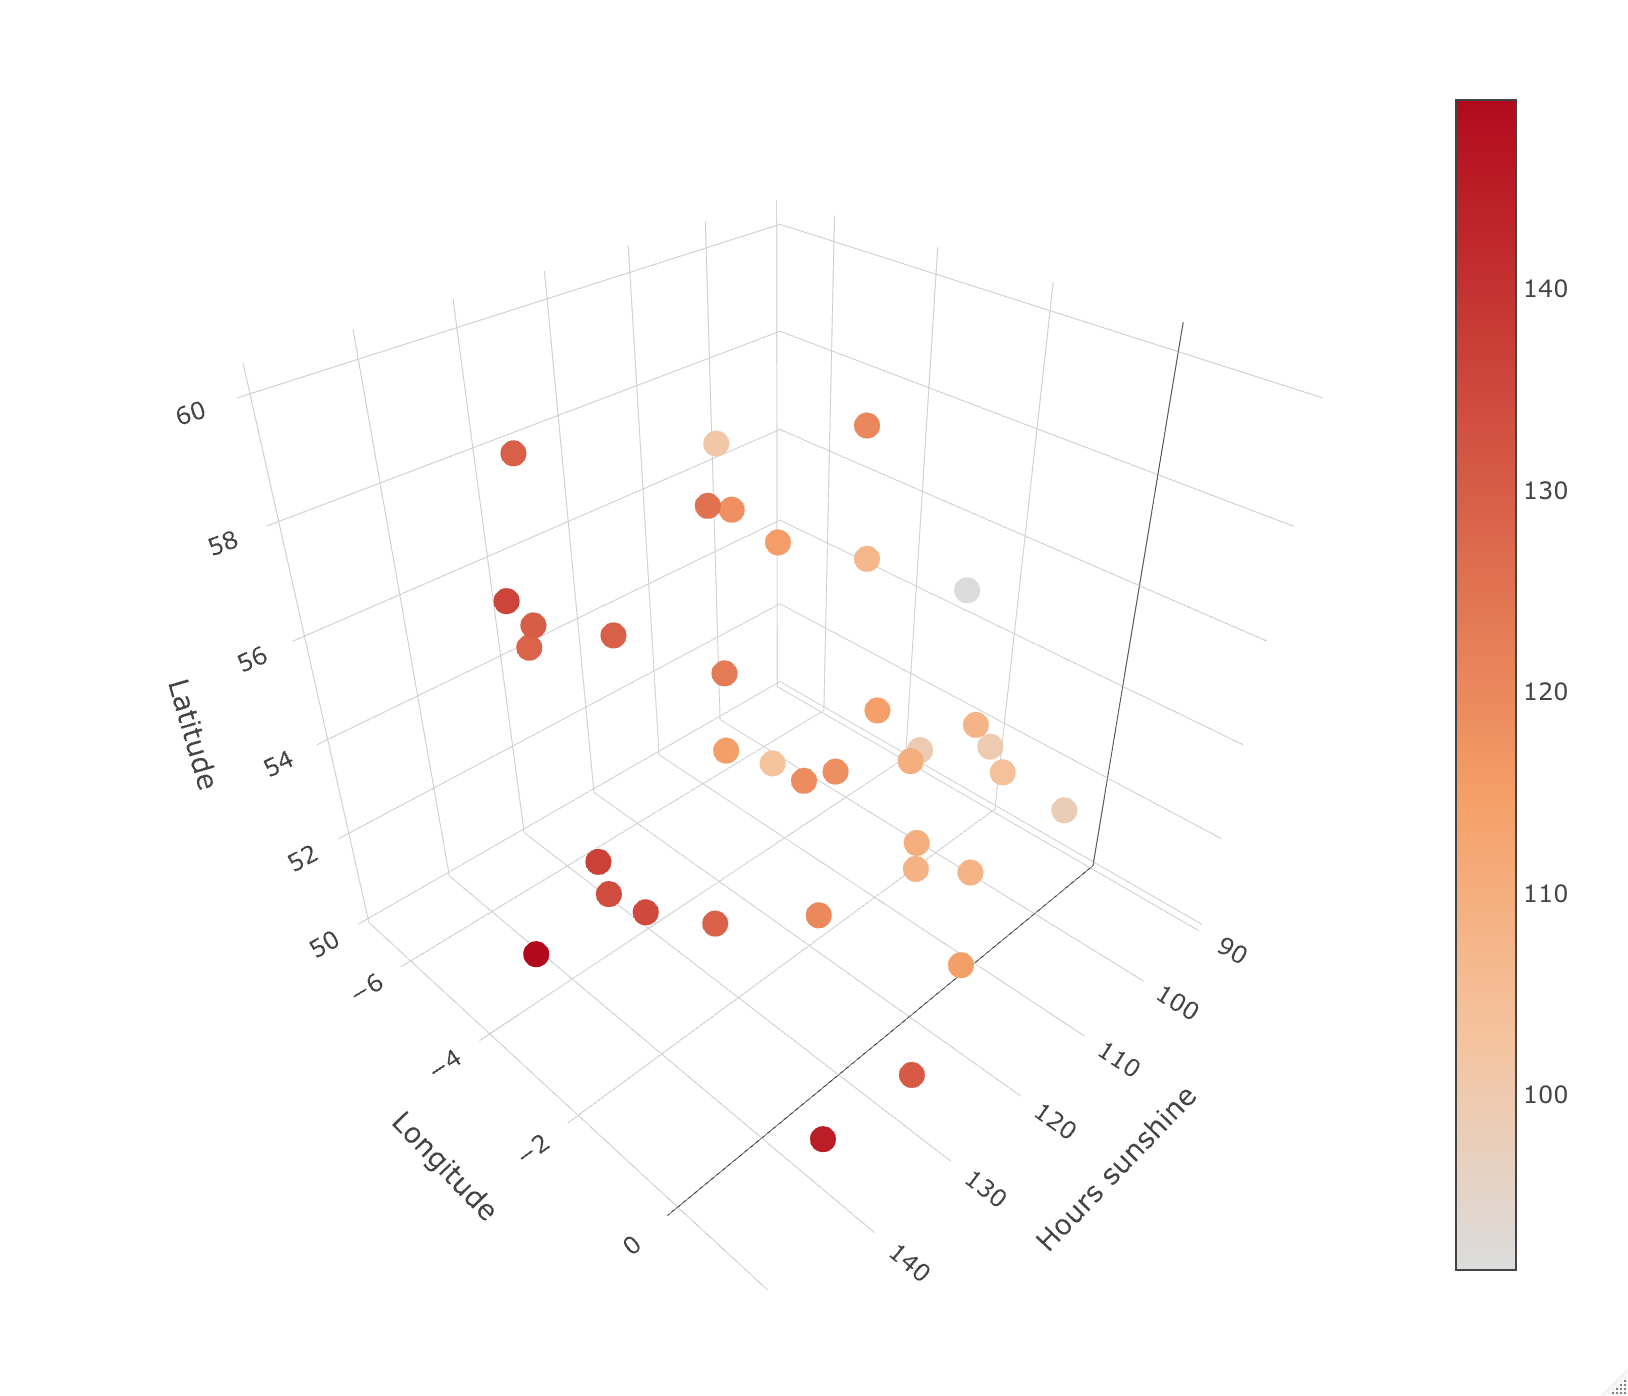
\includegraphics[scale=0.4, trim={6cm 0 0 0},clip]{question_1_014_eda_charts_longitude_latitude_hours_sun}
	\caption{Mean hours of sunshine per weather station by latitude and longitude}
	\label{fig:question_1_014_eda_charts_longitude_latitude_hours_sun}
\end{figure}

\begin{figure}
	\centering
	\captionsetup{justification=centering}
	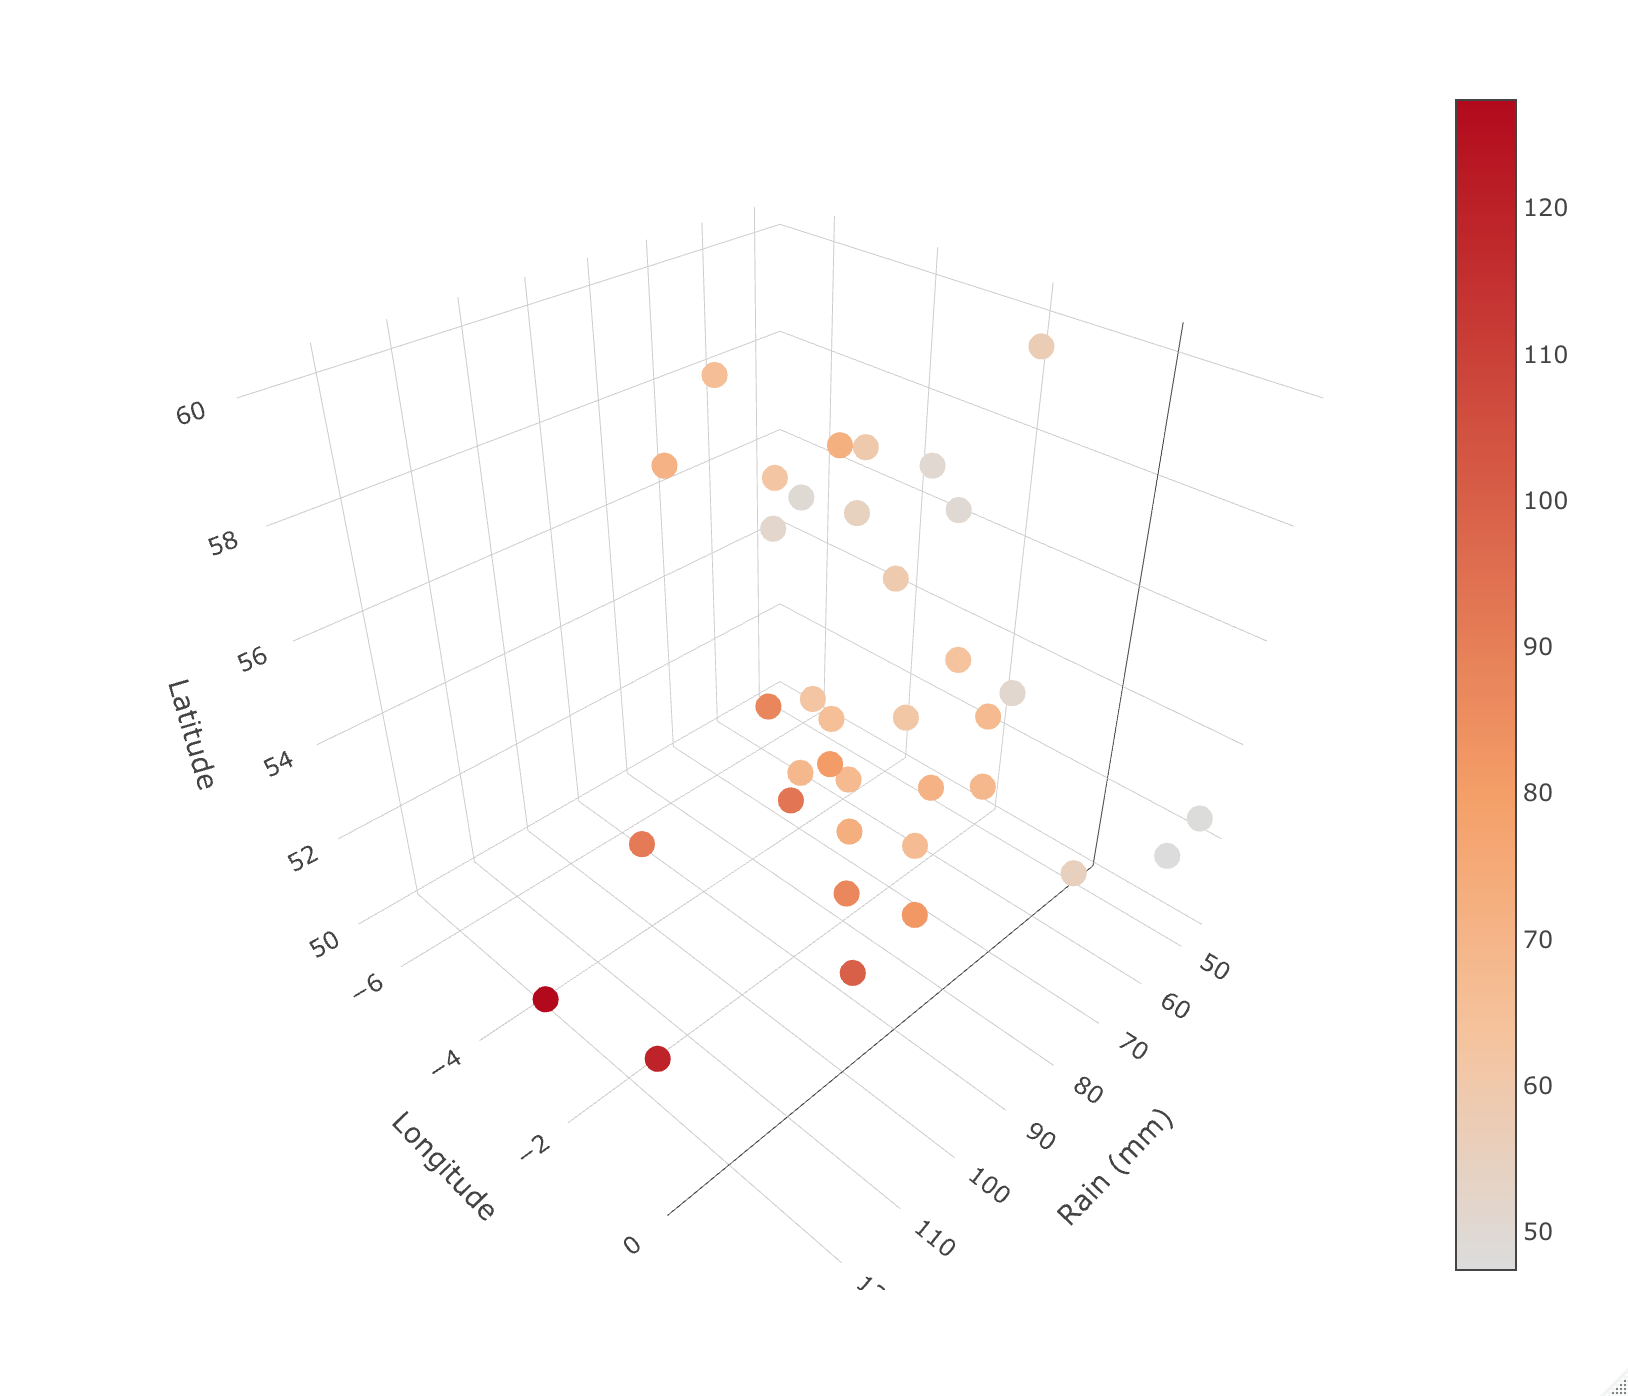
\includegraphics[scale=0.4, trim={6cm 0 0 0},clip]{question_1_015_eda_charts_latitude_longitude_rain_mm}
	\caption{Mean rain (mm) per weather station by latitude and longitude}
	\label{fig:question_1_015_eda_charts_longitude_latitude_rain_mm}
\end{figure}

\begin{figure}
	\centering
	\captionsetup{justification=centering}
	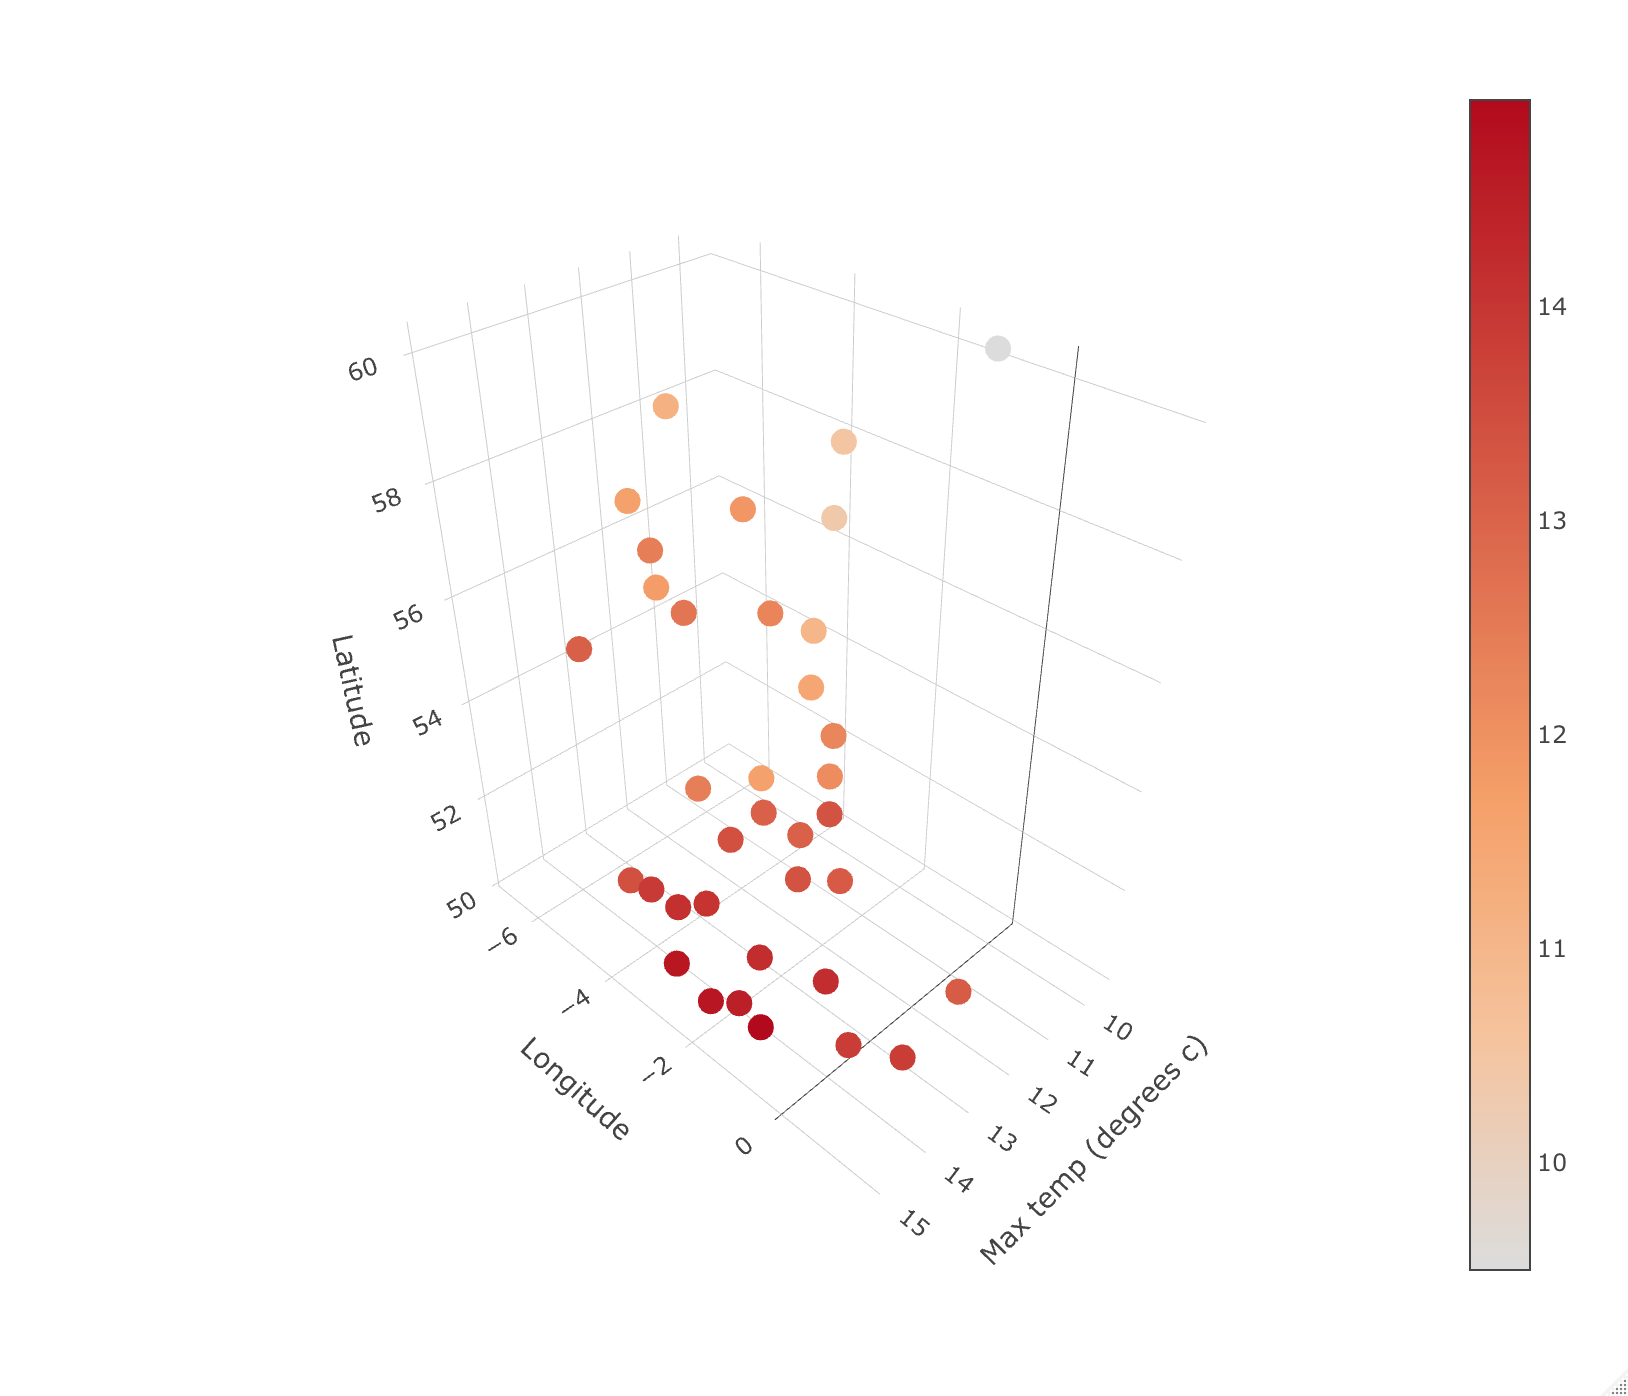
\includegraphics[scale=0.4, trim={6cm 0 0 0},clip]{question_1_016_eda_charts_latitude_longitude_max_temp}
	\caption{Mean max temperature (degrees c) per weather station by latitude and longitude}
	\label{fig:question_1_016_eda_charts_latitude_longitude_max_temp}
\end{figure}

\begin{figure}
	\centering
	\captionsetup{justification=centering}
	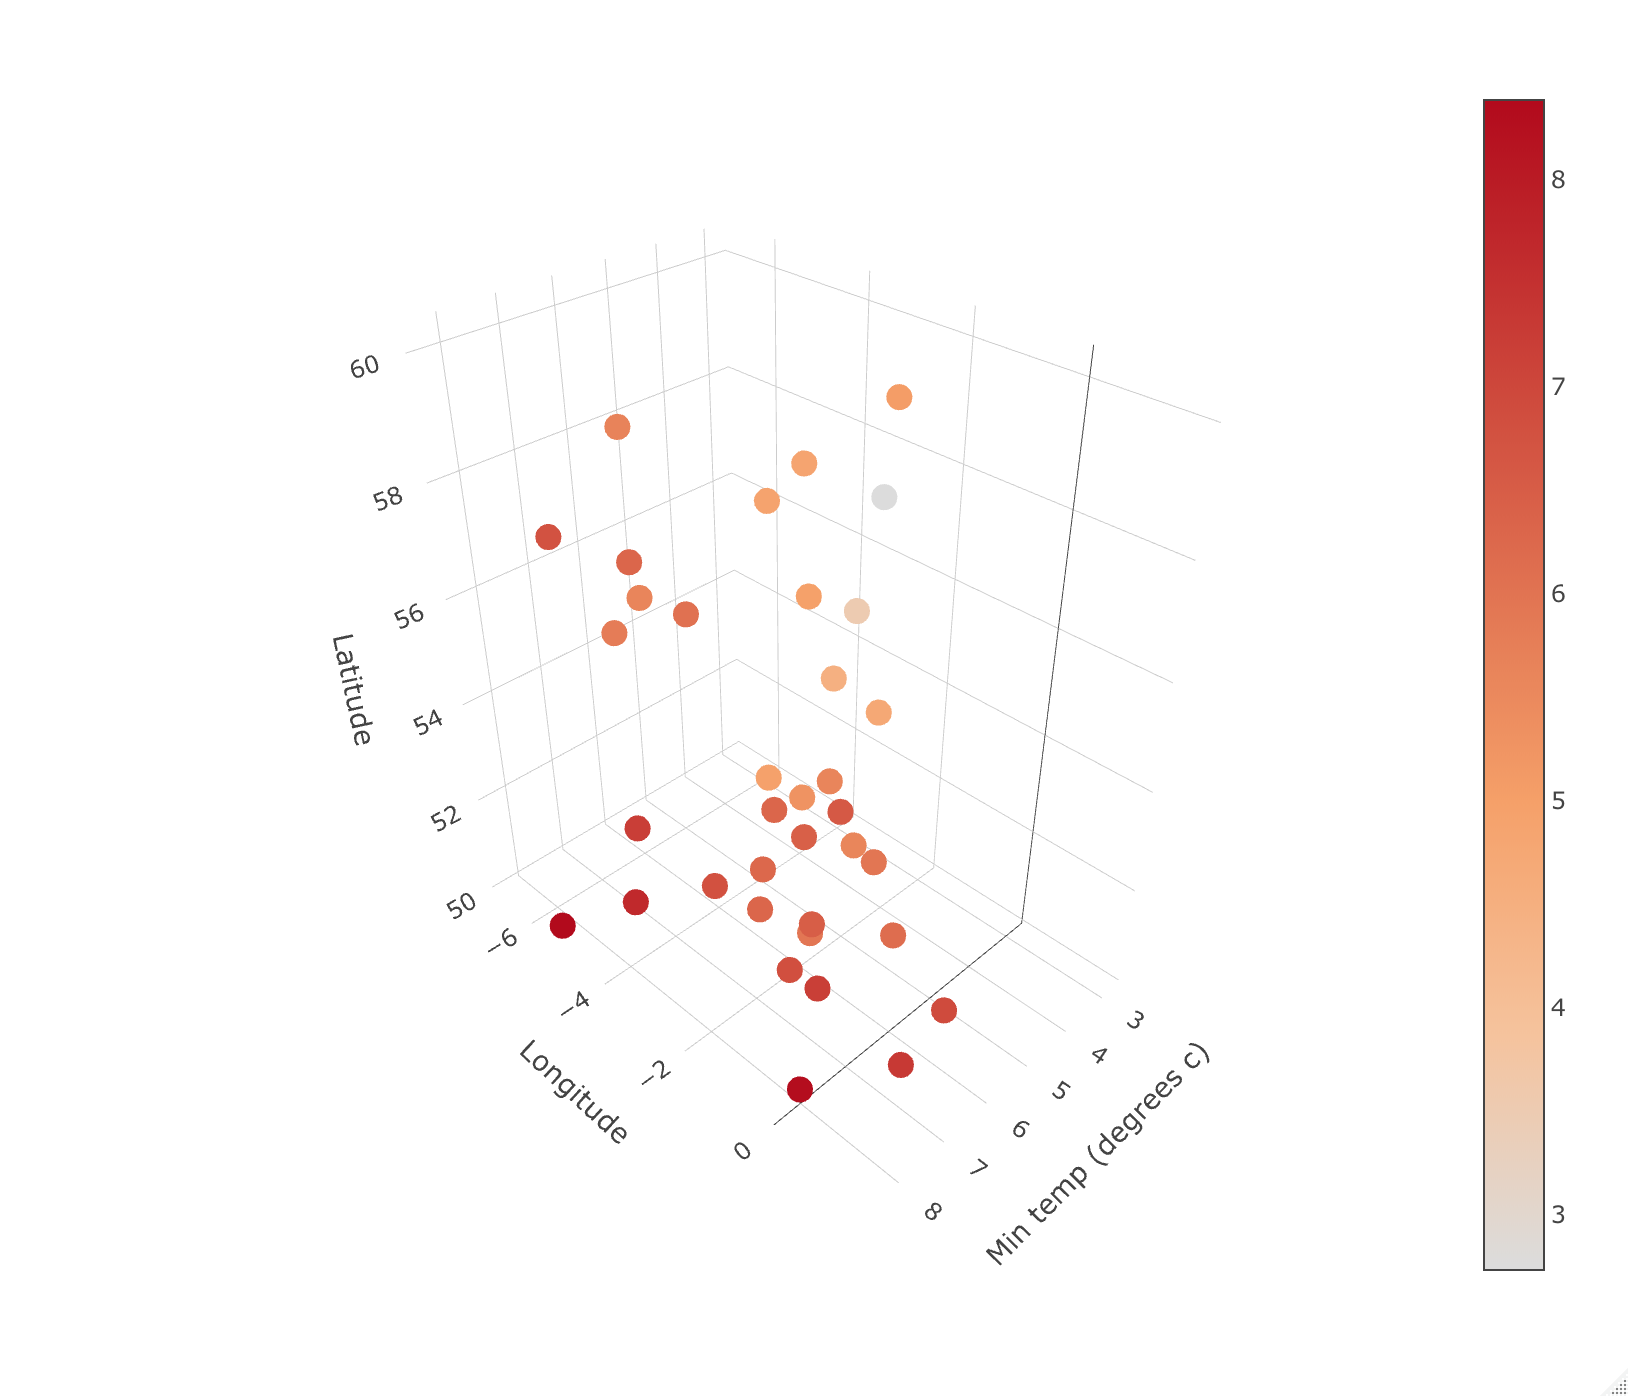
\includegraphics[scale=0.4, trim={6cm 0 0 0},clip]{question_1_017_eda_charts_longitude_latitude_min_temp}
	\caption{Mean min temperature (degrees c) per weather station by latitude and longitude}
	\label{fig:question_1_017_eda_charts_longitude_latitude_min_temp}
\end{figure}

\bigskip
\begin{lstlisting}
pids.wellbeing.weather::

question_1_014_eda_charts_longitude_latitude_hours_sun()
question_1_015_eda_charts_longitude_latitude_rain_mm()
question_1_016_eda_charts_longitude_latitude_max_temp()
question_1_017_eda_charts_longitude_latitude_min_temp()
\end{lstlisting}

\subsection*{Cluster tendency}
\addcontentsline{toc}{subsection}{Cluster tendency}
The clustering tendency of the data has been calculated using the Hopkins statistic (H). It assesses the probability that the data contains non random structures. The statistic has been calculated using the \emph{factoextra} dependency. Using the data with outliers removed, the result of H was \textbf{0.352}. When H > 0.5 it is unlikely that the associated data contains significant clusters. Consequently, the found value of H accords with the intuitive understanding (from Figures \ref{fig:question_1_014_eda_charts_longitude_latitude_hours_sun},  \ref{fig:question_1_015_eda_charts_longitude_latitude_rain_mm}, \ref{fig:question_1_016_eda_charts_latitude_longitude_max_temp} and \ref{fig:question_1_017_eda_charts_longitude_latitude_min_temp}) that the data contain clusters. This suggestion will be further examined with regard to the development of a VAT chart, as described below.

The function used to generate this H statistic can be run using the command below:
\bigskip
\begin{lstlisting}
pids.wellbeing.weather::

question_1_018_prep_cluster_tendency()
question_1_018_prep_cluster_tendency(show_chart = TRUE)
\end{lstlisting}

\subsection*{VAT}
\addcontentsline{toc}{subsection}{VAT}
Figure \ref{fig:question_1_019_prep_charts_vat} illustrates a VAT chart of variables by weater station. It was produced using the \emph{factoextra} package, and it can be run using the command below.
\color{red}The text above is not complete\color{black}

\bigskip
\begin{figure}
	\centering
	\captionsetup{justification=centering}
	\includegraphics[scale=0.4]{question_1_019_prep_charts_vat}
	\caption{VAT chart of the weather variables grouped by weather station}
	\label{fig:question_1_019_prep_charts_vat}
\end{figure}

\bigskip
\begin{lstlisting}
pids.wellbeing.weather::question_1_019_prep_charts_vat()
\end{lstlisting}

\section*{Data preparation}
\addcontentsline{toc}{section}{Data preparation}

\subsection*{K choice}
\addcontentsline{toc}{subsection}{K choice}
K is a variable that describes the number of clusters into which a dataset should be organised. It is used with a number of machine learning algorithms, including K Means. In order to auotmate the generation of the clusters for question 1, an optimum value of K was found using the NbClust package, as used within the \emph{question\_1\_020\_prep\_k\_choice} exported function. The function searched for values of K from two to ten and did so for several potential clustering types: \emph{centroid}, \emph{average}, \emph{complete}, and \emph{kmeans}. This function can be run with default parameters and doing do returns the interger value of the optimim value of K. In contrast, the function can be run with the \emph{verbose} parameter equal to TRUE. This returns a detailed output, as can be seen within Figure \ref{fig:question_1_020_prep_k_choice_console_output}.

\begin{figure}
	\centering
	\captionsetup{justification=centering}
	\includegraphics[scale=0.5]{question_1_020_prep_k_choice_console_output}
	\caption{Console output from function \emph{question\_1\_020\_prep\_k\_choice}}
	\label{fig:question_1_020_prep_k_choice_console_output}
\end{figure}

\bigskip
\begin{lstlisting}
pids.wellbeing.weather::

question_1_020_prep_k_choice()
question_1_020_prep_k_choice(verbose = TRUE)
\end{lstlisting}

\subsection*{Algorithm choice}
\addcontentsline{toc}{subsection}{Algorithm choice}
Figure \ref{fig:question_1_021_prep_algorithm_choice_console_ouput} illustrates the console output from the automated algorithm choice function, \emph{question\_1\_021\_prep\_algorithm\_choice}, which can be called using the command below, and which makes use of the clValid library.

\color{red}The text above is not complete\color{black}

\begin{figure}
	\centering
	\captionsetup{justification=centering}
	\includegraphics[scale=0.6]{question_1_021_prep_algorithm_choice_console_ouput}
	\caption{Console output from function \emph{}question\_1\_021\_prep\_algorithm\_choice}
	\label{fig:question_1_021_prep_algorithm_choice_console_ouput}
\end{figure}

\bigskip
\begin{lstlisting}
pids.wellbeing.weather::question_1_021_prep_algorithm_choice()
\end{lstlisting}

\subsection*{Linkage choice}
\addcontentsline{toc}{subsection}{Linkage choice}
Table \ref{table:question_1_022_prep_linkage_choice} summarises the output from the automated linkage choice function, \emph{question\_1\_022\_prep\_linkage\_choice}, which can be called using the command below, and which makes use of the \emph{cluster} library.
\color{red}The text above is not complete\color{black}

\begin{table}[h!]
	\centering
	\begin{tabular}{ |c|c|c| }
		\hline
		Distance Type & Linkage Type & Cophenetic (3sf) \\
		\hline
		\hline
		 euclidean  &  average   &  0.676 \\
		manhattan  &  average  & 0.664 \\
		euclidean & ward.D2  & 0.596 \\
		euclidean  & complete   & 0.595 \\		
		 manhattan  & centroid  & 0.578 \\
		euclidean  & centroid  & 0.564 \\
		 manhattan & ward.D2  & 0.538 \\
		euclidean  & ward.D   & 0.525 \\		
		manhattan  & ward.D   & 0.483 \\
		euclidean  & single  & 0.465 \\
		manhattan & complete  & 0.445 \\
		manhattan  & single   & 0.370 \\
		\hline
	\end{tabular}
	\caption{Cophenetic values (3sf) per distance and linkage type.}
	\label{table:question_1_022_prep_linkage_choice}
\end{table}

\bigskip
\begin{lstlisting}
pids.wellbeing.weather::question_1_022_linkage_choice()
\end{lstlisting}

\section*{Analysis}
\addcontentsline{toc}{section}{Analysis}

\subsection*{Hierarchical}
\addcontentsline{toc}{subsection}{Hierarchical}
Using the linkage and distance values defined above, a hierarchical cluster was produced by the exported function \emph{question\_1\_023\_analysis\_hierarchical}. The exported function \emph{question\_1\_025\_analysis\_attach\_pruned\_cluster\_values} produced pruned hierarchical cluster, using K = 3, and a dendrographic representation of the pruned cluster was produced by exported function \emph{question\_1\_024\_analysis\_charts\_dendrogram}, as can be seen within Figure \ref{fig:question_1_024_analysis_charts_dendrogram}. 
\color{red}The text above is not complete\color{black}

\begin{figure}
	\centering
	\captionsetup{justification=centering}
	\includegraphics[scale=0.7]{question_1_024_analysis_charts_dendrogram}
	\caption{Hierarchical cluster dendrograph of weather featues with K = 3}
	\label{fig:question_1_024_analysis_charts_dendrogram}
\end{figure}

\bigskip
\begin{lstlisting}
pids.wellbeing.weather::

question_1_023_analysis_hierarchical()
question_1_024_analysis_charts_dendrogram()
question_1_025_analysis_attach_pruned_cluster_values()
\end{lstlisting}


\subsection*{k-means}
\addcontentsline{toc}{subsection}{K-means}
The exported function \emph{question\_1\_026\_analysis\_kmeans} ran K-means multiple times across the weather features using values of K between one and ten. The resulting \emph{sum of squares} chart can be run using the exported function,  described below, and the ouput can be seen within Figure \ref{fig:question_1_027_analysis_charts_sum_squares}.
\color{red}The text above is not complete\color{black}

\begin{figure}
	\centering
	\captionsetup{justification=centering}
	\includegraphics[scale=0.7]{question_1_027_analysis_charts_sum_squares}
	\caption{K Means sum of squares for value of K up to 10.}
	\label{fig:question_1_027_analysis_charts_sum_squares}
\end{figure}

\bigskip
\begin{lstlisting}
pids.wellbeing.weather::

question_1_026_analysis_kmeans()
question_1_027_analysis_charts_sum_squares()
\end{lstlisting}

\section*{Evaluation}
\addcontentsline{toc}{section}{Evaluation}

\subsection*{Hierarchical cluster results by latitude}
\addcontentsline{toc}{subsection}{Hierarchical cluster results by latitude}
The evaluation of the hierarchical cluster can begin by comparing the results with regard to latitude. Such a comparison can be generated by the  using the exported function described below, which used the \emph{ggplot2} and \emph{gridExtra} libraries, and whose output can be seen within Figure \ref{fig:question_1_032_eval_charts_hierarchical_latitude}.
\color{red}The text above is not complete\color{black}.

\begin{figure}
	\centering
	\captionsetup{justification=centering}
	\includegraphics[scale=0.7]{question_1_032_eval_charts_hierarchical_latitude}
	\caption{Weather stations by latitude with hierarchical cluster group s(k = 3).}
	\label{fig:question_1_032_eval_charts_hierarchical_latitude}
\end{figure}

\bigskip
\begin{lstlisting}
pids.wellbeing.weather::question_1_032_eval_charts_hierarchical_latitude()
\end{lstlisting}

\subsection*{Hierarchical cluster results by latitude and longitude}
\addcontentsline{toc}{subsection}{Hierarchical cluster results by longitude}

\begin{figure}
	\centering
	\captionsetup{justification=centering}
	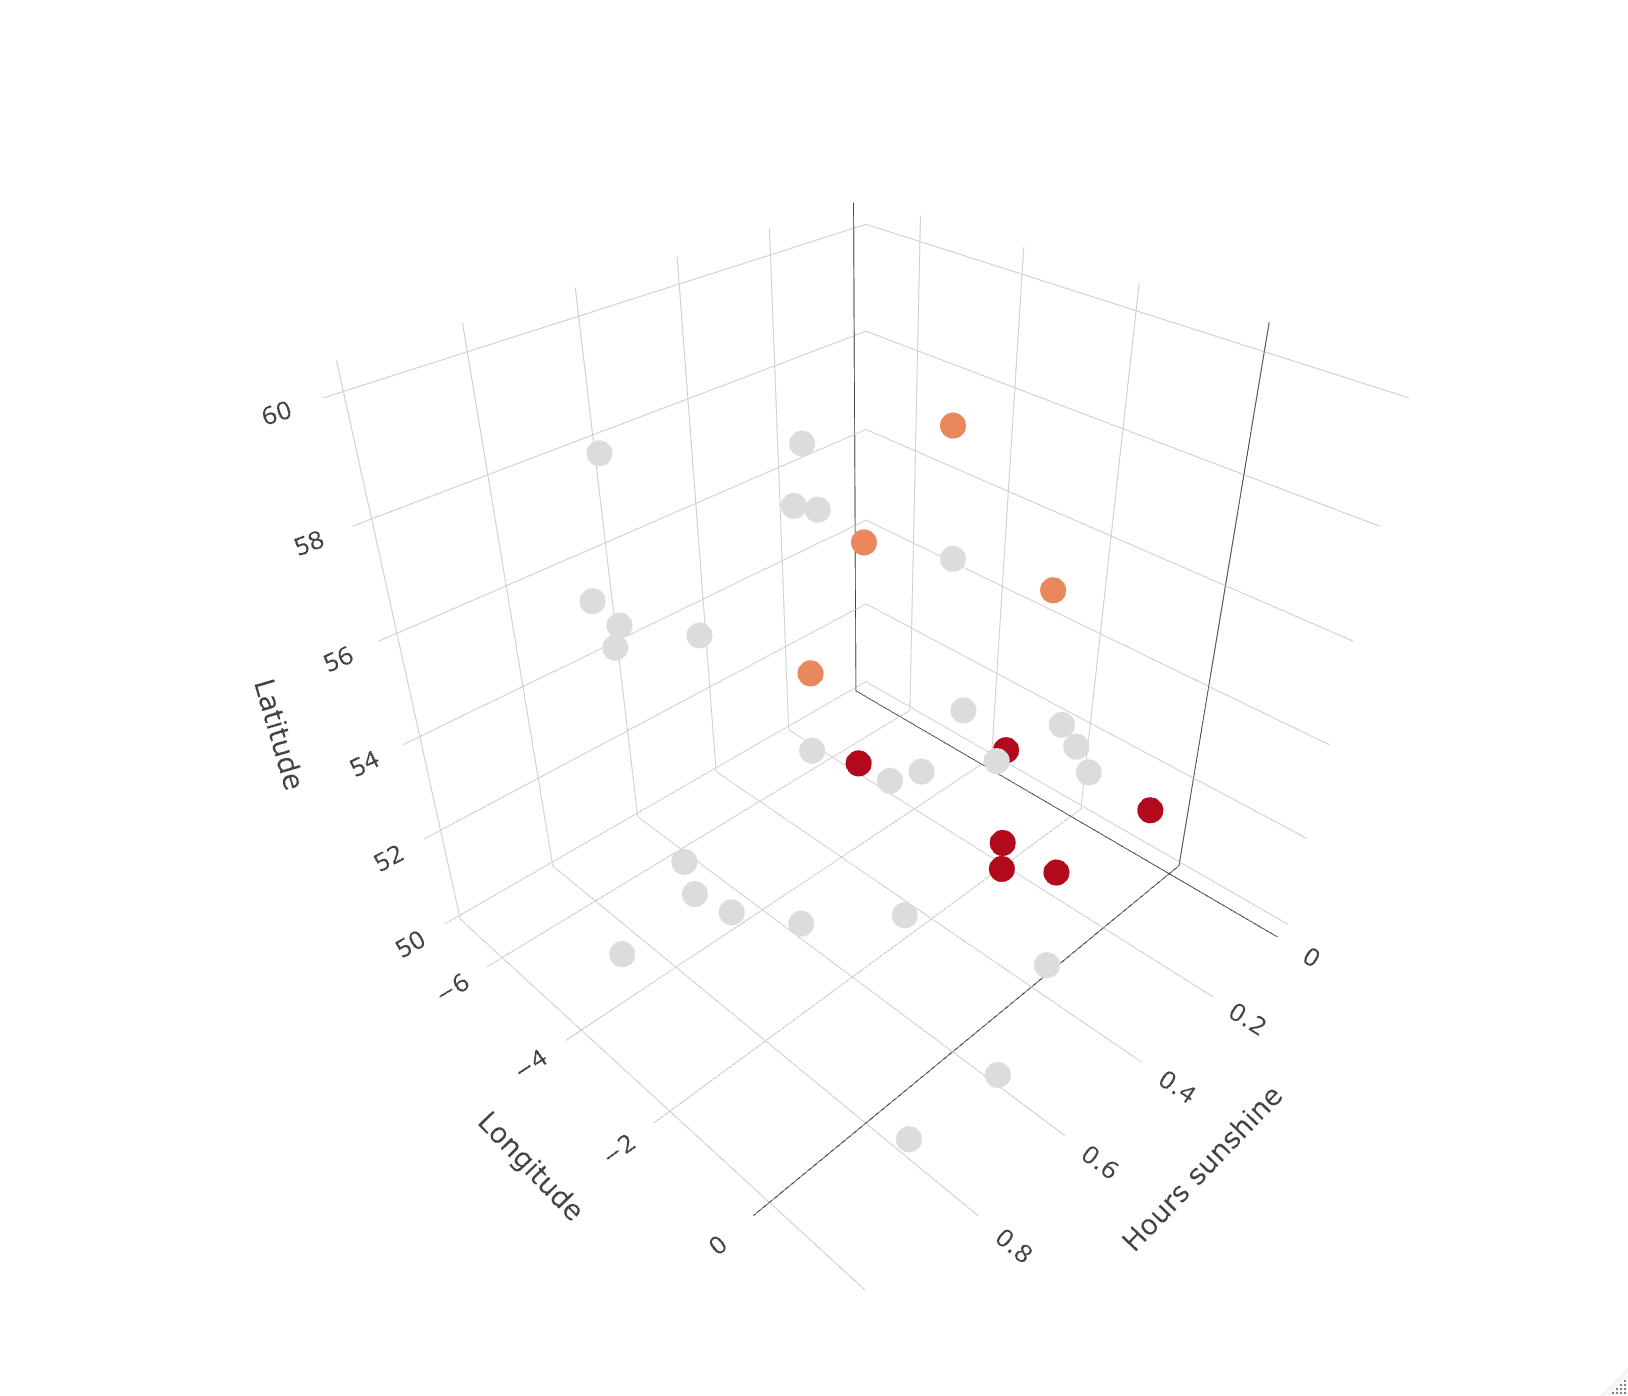
\includegraphics[scale=0.4, trim={8cm 0 0 0},clip]{question_1_033_eval_charts_hier_latitude_longitude_hours_sun}
	\caption{Hours sunshine per weather stations by latitude and longitude with hierarchical cluster groups (k = 3).}
	\label{fig:question_1_033_eval_charts_hier_latitude_longitude_hours_sun}
\end{figure}

\begin{figure}
	\centering
	\captionsetup{justification=centering}
	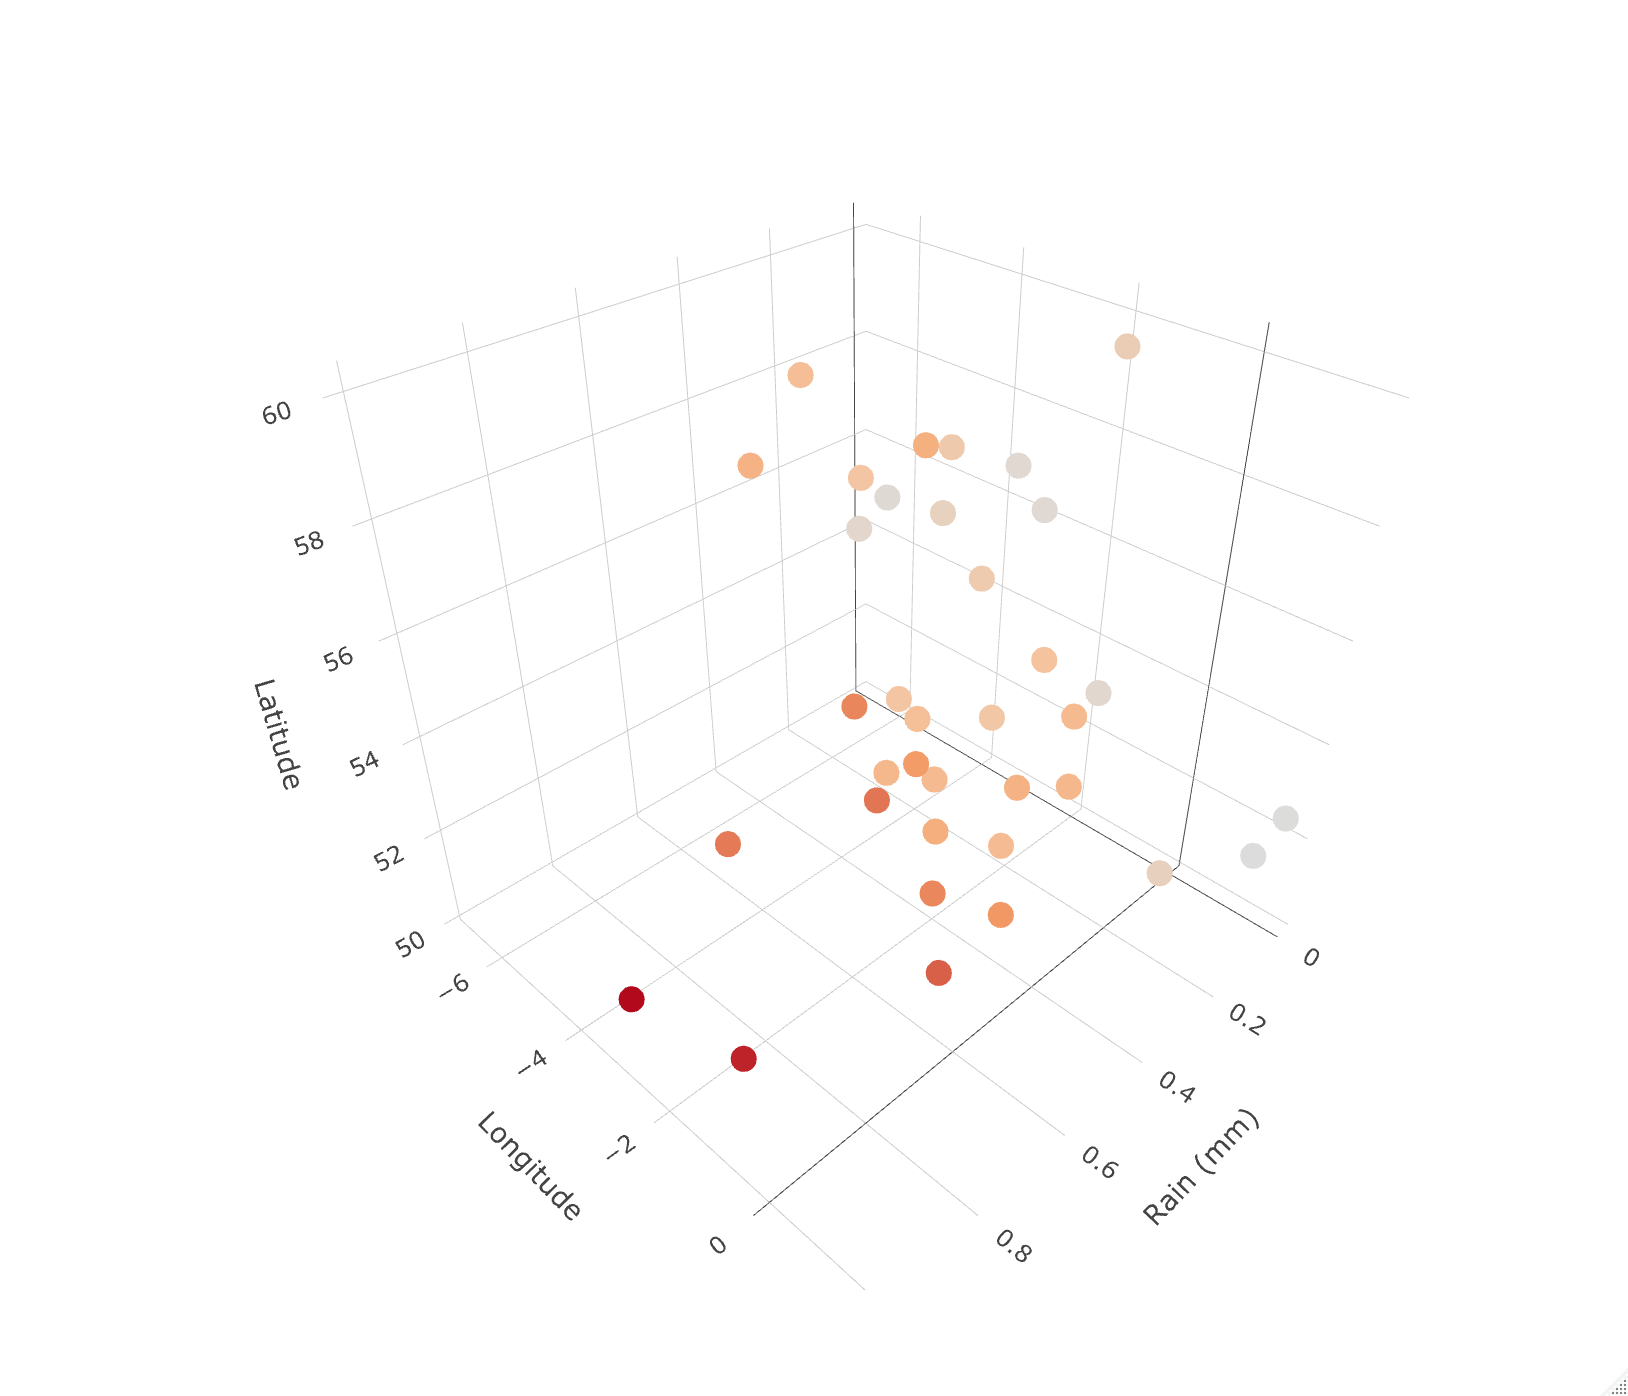
\includegraphics[scale=0.4, trim={8cm 0 0 0},clip]{question_1_034_eval_charts_hier_latitude_longitude_rain_mm}
	\caption{Rain (mm) per weather stations by latitude and longitude with hierarchical cluster groups (k = 3).}
	\label{fig:question_1_034_eval_charts_hier_latitude_longitude_rain_mm}
\end{figure}

\begin{figure}
	\centering
	\captionsetup{justification=centering}
	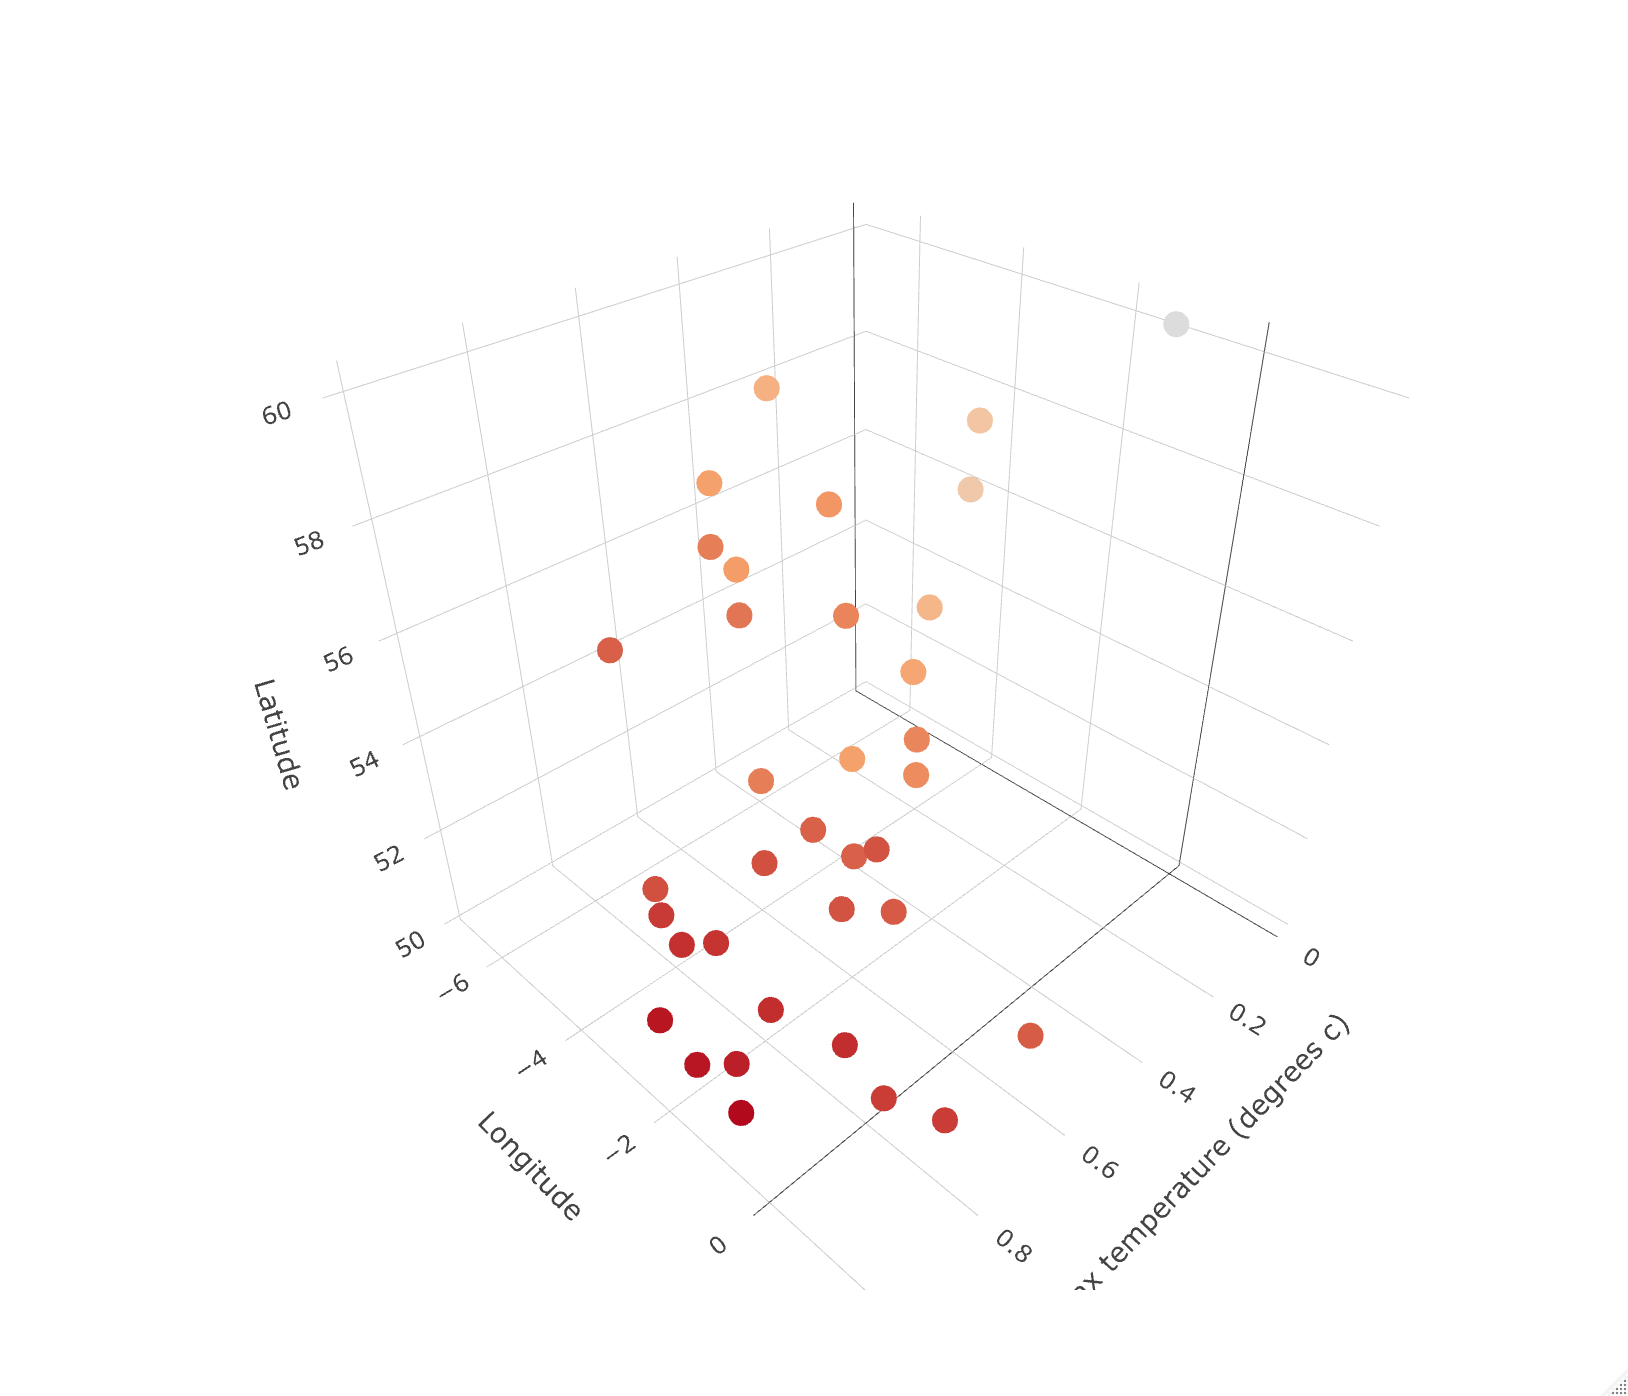
\includegraphics[scale=0.4, trim={8cm 0 0 0},clip]{question_1_035_eval_charts_hier_latitude_longitude_max_temp}
	\caption{Max temperatuer (degrees c) per weather stations by latitude and longitude with hierarchical cluster groups (k = 3).}
	\label{fig:question_1_035_eval_charts_hier_latitude_longitude_max_temp}
\end{figure}

\begin{figure}
	\centering
	\captionsetup{justification=centering}
	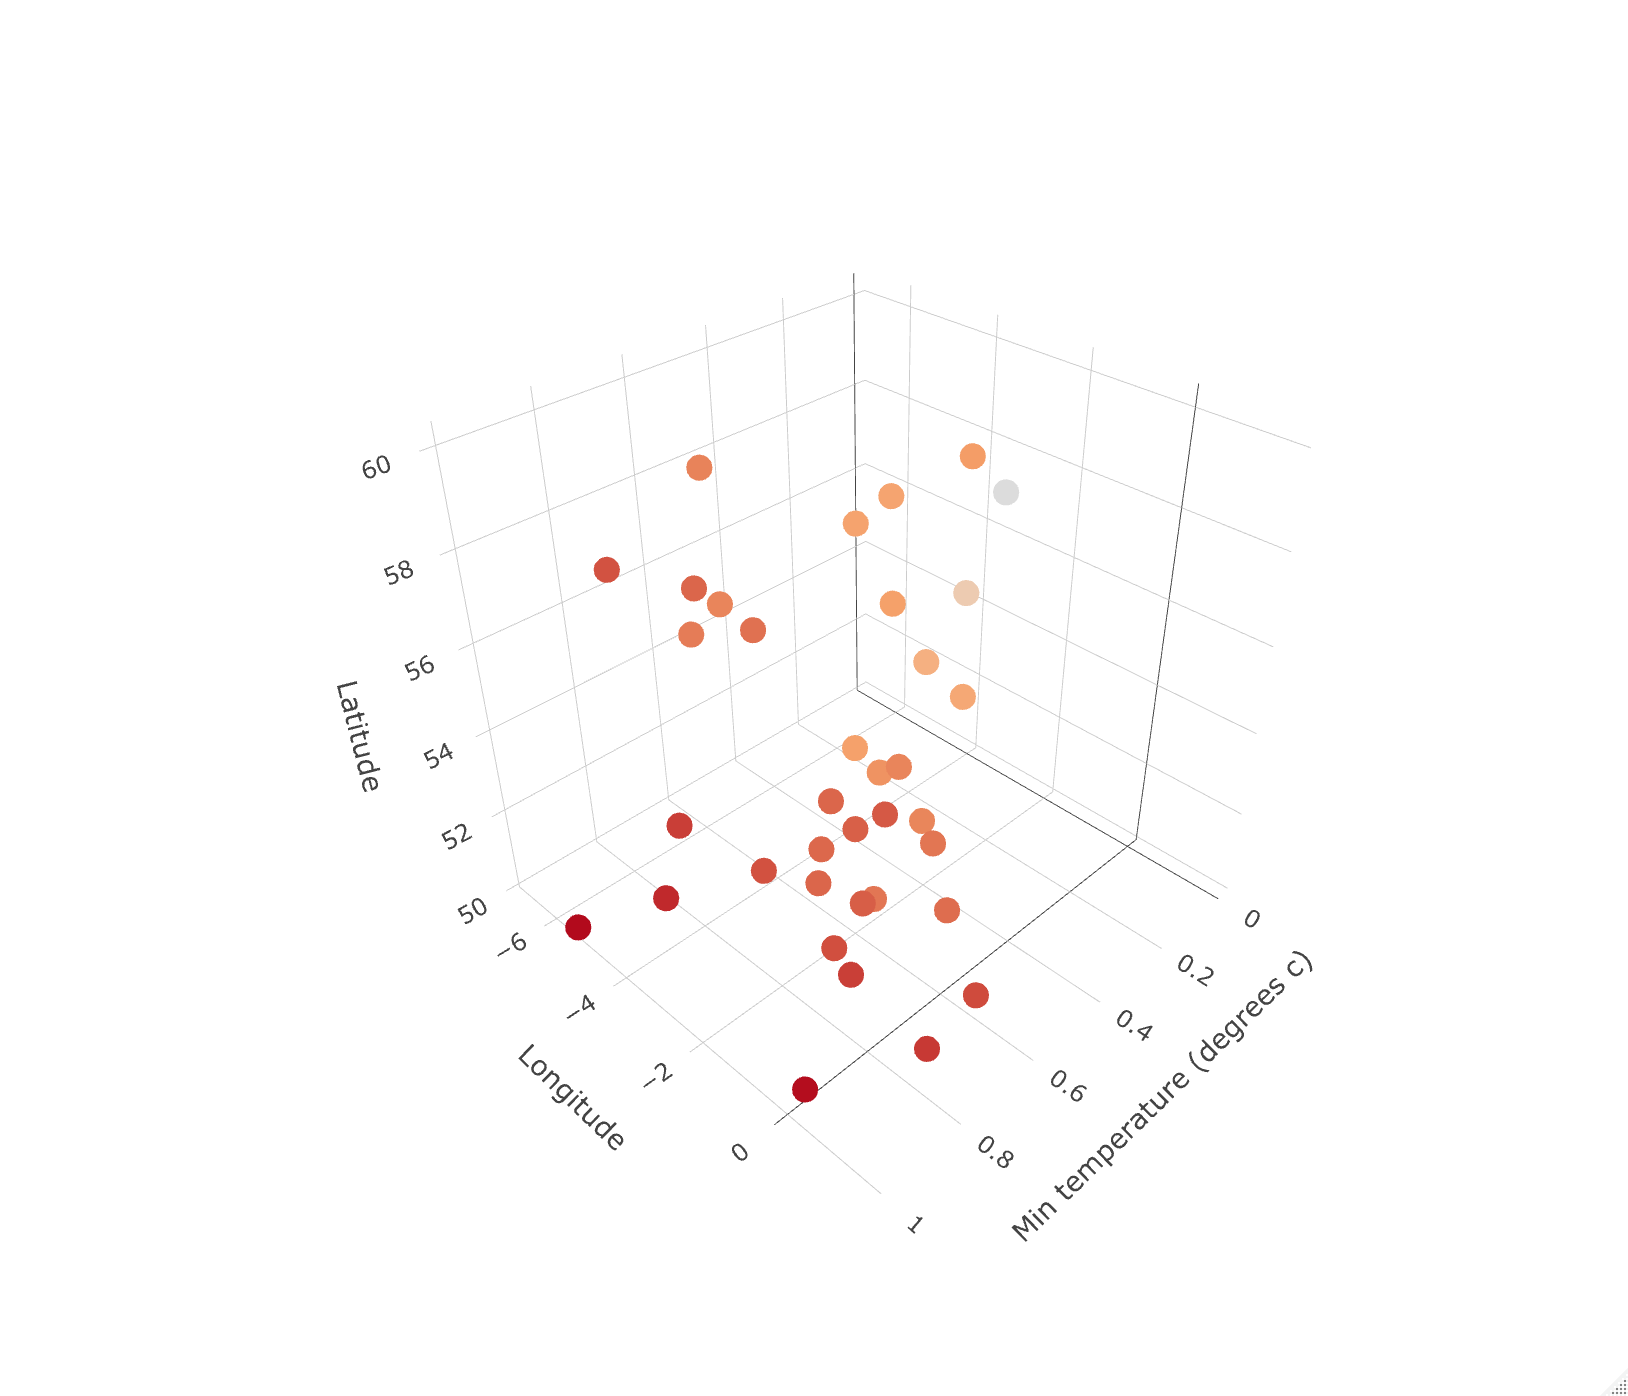
\includegraphics[scale=0.4, trim={8cm 0 0 0},clip]{question_1_036_eval_charts_hier_latitude_longitude_min_temp}
	\caption{Min temperatuer (degrees c) per weather stations by latitude and longitude with hierarchical cluster groups (k = 3).}
	\label{fig:question_1_036_eval_charts_hier_latitude_longitude_min_temp}
\end{figure}

\bigskip
\begin{lstlisting}
pids.wellbeing.weather::

question_1_033_eval_charts_hier_latitude_longitude_hours_sun()
question_1_034_eval_charts_hier_latitude_longitude_rain_mm()
question_1_035_eval_charts_hier_latitude_longitude_max_temp()
question_1_036_eval_charts_hier_latitude_longitude_min_temp()
\end{lstlisting}

\section*{Deployment}
\addcontentsline{toc}{section}{Deployment}
\color{red}The description of the automated deployment process is not complete. However, the function described below is complete.\color{black}
\begin{lstlisting}
#' question_1_037_automated
#' @export
question_1_037_automated <- function() {
	question_1_001_svc_raw_data()
	question_1_002_svc_tech_weather_txt()
	question_1_003_svc_tech_weather_dsv()
	question_1_004_svc_tech_weather_df()
	question_1_005_svc_tech_weather_complete()
	question_1_006_svc_tech_weather_single_df()
	question_1_008_svc_cons_grouped_data()
	question_1_011_eda_remove_outliers()
	k_value <- question_1_020_prep_k_choice()
	question_1_025_analysis_attach_pruned_cluster_values(
		k_value = k_value
	)
}
\end{lstlisting}

\bigskip
\begin{lstlisting}
pids.wellbeing.weather::question_1_037_automated()
\end{lstlisting}

\setcounter{equation}{0}
\chapter*{Question 2}
\addcontentsline{toc}{chapter}{Question 2}

\section*{Data Understanding}
\addcontentsline{toc}{section}{Data Understanding}

\subsection*{Append latitude categories}
\addcontentsline{toc}{subsection}{Append latitude categories}

Latitude categories were appended to the grouped, cleaned data (with ouliers removed) by the exported function \emph{question\_2\_001\_bu\_append\_latitude\_categorie}, which made use of the latutude category boundaries illustrated within Table \ref{table:question_2_001_bu_append_latitude_categories}. The command provided within Listing \ref{lst:question_2_001_bu_append_latitude_categories} can be used to run this function.
\color{red}The text above is not complete\color{black}.

\begin{table}[ht]
	\centering
	\begin{tabular}{rlr|r}
		\hline
		& Latitude category & Lower boundary & Upper boundary \\ 
		\hline
		1 & bottom &  49.9 & 53.567  \\ 
		2 & middle &  53.567 & 57.234 \\ 
		3 & top &  57.234 & 60.9 \\ 
		\hline
	\end{tabular}
	\caption{Upper and lower latitude category boundaries}
	\label{table:question_2_001_bu_append_latitude_categories}
\end{table}

	
\bigskip
\begin{lstlisting}[caption=Command to append latitude categories., label={lst:question_2_001_bu_append_latitude_categories}]
pids.wellbeing.weather::question_2_001_bu_append_latitude_categories
\end{lstlisting}

\subsection*{Exploratory data analysis (EDA)}
\addcontentsline{toc}{subsection}{Exploratory data analysis (EDA)}

\subsubsection*{Number of weather stations per latitude category}
\addcontentsline{toc}{subsubsection}{Number of weather stations per latitude category}

\begin{table}[ht]
\centering
\begin{tabular}{rlr}
  \hline
 & latitude\_category & n \\ 
  \hline
1 & bottom &  20 \\ 
  2 & middle &  12 \\ 
  3 & top &   4 \\ 
   \hline
\end{tabular}
\end{table}

\bigskip
\begin{lstlisting}[escapeinside={(*}{*)}]
pids.wellbeing.weather::

question_2_002_eda_latitude_category_summary()$nrow
question_2_002_eda_latitude_category_summary()$weather_stations
\end{lstlisting}

\subsubsection*{Mean weather features per latitude category}
\addcontentsline{toc}{subsubsection}{Mean weather features per latitude category}
\bigskip


\begin{figure}
	\centering
	\captionsetup{justification=centering}
	\includegraphics[scale=0.7]{question_2_003_eda_charts_weather_features}
	\caption{Mean weather features per latitude category.}
	\label{fig:question_2_003_eda_charts_weather_features}
\end{figure}

\begin{table}[ht]
\centering
\begin{tabular}{rlrrrr}
  \hline
 & latitude\_category & hours\_sun & rain\_mm & temp\_max\_degrees\_c & temp\_min\_degrees\_c \\ 
  \hline
1 & bottom & 0.47 & 0.34 & 0.77 & 0.69 \\ 
  2 & middle & 0.44 & 0.20 & 0.46 & 0.45 \\ 
  3 & top & 0.55 & 0.20 & 0.23 & 0.42 \\ 
   \hline
\end{tabular}
\end{table}

\begin{lstlisting}[escapeinside={(*}{*)}]
pids.wellbeing.weather::

question_2_002_eda_latitude_category_summary()$means
question_2_003_eda_charts_weather_features()
\end{lstlisting}

\subsubsection*{Latitude category pairwise comparisons}
\addcontentsline{toc}{subsubsection}{Latitude category pairwise comparisons}
\color{red}Description not complete\color{black}.
\bigskip
\begin{lstlisting}
pids.wellbeing.weather::question_2_004_eda_charts_latitude_category_pairwise()
\end{lstlisting}

\subsubsection*{Latitude and longitude per latitude category}
\addcontentsline{toc}{subsubsection}{Latitude and longitude per latitude category}
\color{red}Description not complete\color{black}.
\bigskip
\begin{lstlisting}
pids.wellbeing.weather::

question_2_005_eda_charts_latitude_longitude_hours_sun()
question_2_005_eda_charts_latitude_longitude_rain()
question_2_005_eda_charts_latitude_longitude_temp_max
question_2_005_eda_charts_latitude_longitude_temp_min
\end{lstlisting}

\section*{Data Preparation}
\addcontentsline{toc}{section}{Data Preparation}

\subsubsection*{Training and test data split}
\addcontentsline{toc}{subsubsection}{Training and test data split}
\color{red}Description not complete\color{black}.
\bigskip
\begin{lstlisting}
pids.wellbeing.weather::question_2_006_prep_split()
\end{lstlisting}

\subsection*{Algorithm choice}
\addcontentsline{toc}{subsection}{Algorithm choice}
\color{red}Description not complete\color{black}.

\section*{Analysis}
\addcontentsline{toc}{section}{Analysis}

\subsubsection*{K Nearest Neighbours}
\addcontentsline{toc}{subsubsection}{K Nearest Neighbours}
\color{red}Description not complete\color{black}.

\bigskip
\begin{lstlisting}
pids.wellbeing.weather::question_2_007_analysis_knn()
\end{lstlisting}

\section*{Deployment}
\addcontentsline{toc}{section}{Deployment}
\color{red}Description not complete\color{black}.

\begin{lstlisting}
#' question_2_008_automated
#' @export
question_2_008_automated <- function() {
	question_2_001_bu_append_latitude_categories()
	question_2_006_prep_split()
	question_2_007_analysis_knn()
}
\end{lstlisting}

\begin{lstlisting}
pids.wellbeing.weather::question_2_008_automated()
\end{lstlisting}

\setcounter{equation}{0}
\chapter*{Question 3}
\addcontentsline{toc}{chapter}{Question 3}

\section*{Data Understanding}
\addcontentsline{toc}{section}{Data Understanding}

\subsection*{Statistical value chain}
\addcontentsline{toc}{subsection}{Statistical value chain}

\subsubsection*{Technically correct: well-being}
\addcontentsline{toc}{subsubsection}{Technically correct: well-being}
\color{red}Description not complete\color{black}.

\bigskip
\begin{lstlisting}
pids.wellbeing.weather::question_3_001_svc_tech_wellbeing()
\end{lstlisting}

\subsubsection*{Consistently correct: weather and well-being}
\addcontentsline{toc}{subsubsection}{Consistently correct: weather and well-being}

\begin{table}[ht]
\centering
\begin{tabular}{rlrrrrrrr}
  \hline
 & Region & Happy & Sun & Latitude & Long' & Rain & Max T' & Min T' \\ 
  \hline
1 & North E & 35.80 & 0.40 & 54.77 & -1.58 & 0.20 & 0.51 & 0.36 \\ 
  2 & North W & 35.90 & 0.24 & 54.01 & -2.53 & 0.46 & 0.51 & 0.47 \\ 
  3 & York' & 34.60 & 0.36 & 53.89 & -1.30 & 0.29 & 0.61 & 0.62 \\ 
  4 & East Mid' & 35.60 & 0.17 & 53.00 & -0.89 & 0.28 & 0.69 & 0.54 \\ 
  5 & West Mid' & 35.60 & 1.00 & 52.79 & -2.66 & 0.17 & 0.72 & 0.45 \\ 
  6 & East & 35.50 & 0.52 & 52.36 & 0.91 & 0.33 & 0.76 & 0.67 \\ 
  7 & London & 31.90 & 0.29 & 51.48 & -0.45 & 0.43 & 1.00 & 0.79 \\ 
  8 & S' East & 35.70 & 0.52 & 51.05 & -0.96 & 0.30 & 0.86 & 0.76 \\ 
  9 & S' West & 35.30 & 0.43 & 51.06 & -3.67 & 0.53 & 0.83 & 0.78 \\ 
  10 & Wales & 35.70 & 0.50 & 52.09 & -3.21 & 0.30 & 0.59 & 0.62 \\ 
  11 & Scotland & 34.80 & 0.50 & 57.19 & -4.06 & 0.16 & 0.34 & 0.42 \\ 
  12 & NI & 38.10 & 0.66 & 54.77 & -6.40 & 0.04 & 0.53 & 0.52 \\ 
   \hline
\end{tabular}
\end{table}

\bigskip
\begin{lstlisting}
pids.wellbeing.weather::

question_3_002_svc_cons_weather_add_boundaries()
question_3_003_svc_cons_weather_wellbeing_join()
question_3_004_svc_cons_weather_wellbeing_summary()
\end{lstlisting}

\bigskip
\bigskip
\subsection*{Exploratory data analysis (EDA)}
\addcontentsline{toc}{subsection}{Exploratory data analysis (EDA)}
\color{red}Description not complete\color{black}.

\begin{table}[ht]
\centering
\begin{tabular}{rll}
  \hline
 & regions & weather\_stations \\ 
  \hline
1 & scotland & lerwick \\ 
  2 & scotland & wickairport \\ 
  3 & scotland & stornoway \\ 
  4 & scotland & nairn \\ 
  5 & scotland & braemar \\ 
  6 & scotland & tiree \\ 
  7 & scotland & dunstaffnage \\ 
  8 & scotland & leuchars \\ 
  9 & scotland & paisley \\ 
  10 & scotland & eskdalemuir \\ 
  11 & northern\_ireland & ballypatrick \\ 
  12 & north\_east & durham \\ 
  13 & north\_west & newtonrigg \\ 
  14 & yorkshire\_and\_the\_humber & whitby \\ 
  15 & northern\_ireland & armagh \\ 
  16 & yorkshire\_and\_the\_humber & bradford \\ 
  17 & yorkshire\_and\_the\_humber & sheffield \\ 
  18 & north\_west & ringway \\ 
  19 & east\_midlands & waddington \\ 
  20 & east\_midlands & suttonbonington \\ 
  21 & west\_midlands & shawbury \\ 
  22 & east & lowestoft \\ 
  23 & wales & cwmystwyth \\ 
  24 & east & cambridge \\ 
  25 & wales & aberporth \\ 
  26 & south\_west & rossonwye \\ 
  27 & wales & oxford \\ 
  28 & south\_east & cardiff \\ 
  29 & london & heathrow \\ 
  30 & south\_east & manston \\ 
  31 & south\_west & yeovilton \\ 
  32 & south\_west & chivenor \\ 
  33 & south\_east & southampton \\ 
  34 & south\_east & eastbourne \\ 
  35 & south\_east & hurn \\ 
  36 & south\_west & camborne \\ 
   \hline
\end{tabular}
\end{table}

\begin{figure}
	\centering
	\captionsetup{justification=centering}
	\includegraphics[scale=0.55]{question_3_005_eda_charts_wellbeing_by_region}
	\caption{Weather features per happiness by region.}
	\label{fig:question_3_005_eda_charts_wellbeing_by_region}
\end{figure}

\bigskip
\begin{lstlisting}
pids.wellbeing.weather::

question_3_005_eda_charts_wellbeing_by_region()
question_3_006_eda_weather_station_regions()
\end{lstlisting}

\section*{Analysis}
\addcontentsline{toc}{section}{Analysis}
\color{red}Description not complete\color{black}.
\bigskip
\begin{lstlisting}
pids.wellbeing.weather::question_3_007_analysis_regression()
pids.wellbeing.weather::question_3_008_analysis_regression_test()
\end{lstlisting}


\section*{Evaluation}
\addcontentsline{toc}{section}{Evaluation}
\color{red}Description not complete\color{black}.

\begin{table}[ht]
	\centering
	\begin{tabular}{rrrrr}
		\hline
		& Estimate & Std. Error & t value & Pr($>$$|$t$|$) \\ 
		\hline
		(Intercept) & 36.8216 & 2.1474 & 17.15 & 0.0000 \\ 
		hours\_sun & 1.5506 & 2.4080 & 0.64 & 0.5401 \\ 
		rain\_mm & -2.3251 & 4.5468 & -0.51 & 0.6248 \\ 
		temp\_max\_degrees\_c & -4.1569 & 4.2687 & -0.97 & 0.3626 \\ 
		temp\_min\_degrees\_c & 2.1683 & 5.4767 & 0.40 & 0.7040 \\ 
		\hline
	\end{tabular}
\end{table}

\bigskip
\begin{lstlisting}
pids.wellbeing.weather::

question_3_009_eval_regression_summary()
question_3_010_eval_charts_predicted_happinesst()
\end{lstlisting}

\section*{Deployment}
\addcontentsline{toc}{section}{Deployment}
\color{red}Description not complete\color{black}.

\begin{lstlisting}
#' question_3_011_automated
#' @export
question_3_011_automated <- function() {
	question_3_001_svc_tech_wellbeing()
	question_3_002_svc_cons_weather_add_boundarie()
	question_3_003_svc_cons_weather_wellbeing_join()
	question_3_007_analysis_regression()
}
\end{lstlisting}

\begin{lstlisting}
pids.wellbeing.weather::question_2_008_automated()
\end{lstlisting}

\setcounter{equation}{0}
\chapter*{Question 4}
\addcontentsline{toc}{chapter}{Question 4}
\color{red}Description not complete\color{black}.

\begin{lstlisting}
pids.wellbeing.weather::question_1_037_automated()
pids.wellbeing.weather::question_2_008_automated()
pids.wellbeing.weather::question_3_011_automated()
\end{lstlisting}
\pagebreak
\bibliography{references} 
\bibliographystyle{ieeetr}

\chapter*{Appendices}
\addcontentsline{toc}{chapter}{Appendices}

\newpage
\section*{A. Function names and question phases}
\addcontentsline{toc}{section}{Function names and question phase}
\label{appendix:function-names-and-question-phases}

\newpage
\section*{B. Raw data function output}
\addcontentsline{toc}{section}{Raw data function output}
\label{appendix:question_1_001_results}

\begin{figure}
	\centering
	\captionsetup{justification=centering}
	\includegraphics[scale=0.7]{question_1_001_results}
	\caption{Output from function question\_1\_001\_svc\_raw\_data}
\end{figure}

\backmatter
\end{document}
